% !TeX root = main.tex
% !TeX spellcheck = en_GB
% !TeX encoding = UTF-8
%
% LaTeX code inspired by the LaTeX Thesis Template by Manuel Kuehner
% www.bedienhaptik.de/latex-template/
% ---------------------------------------------------------------------------- %
%
% Document class definition and package loading
% ┌────────────────────────────────────────────────────────────────────────────┐
% │ DOCUMENT CLASS AND PAGE GEOMETRY                                           │
% └────────────────────────────────────────────────────────────────────────────┘

\documentclass[
 paper=a4                       % use standard A4 paper size
,fontsize=10pt                  % common are 10pt, 11pt, or 12pt
,BCOR=1.0cm                     % defines the binding correction
,twoside=true                   % defines a left-page / right-page document
,DIV=8                          % defines the page layout
,parskip=false                  % removes vertical distance after paragraphs
,numbers=noendperiod            % no dot after last chapter number
,toc=bib                        % bibliography in ToC
,toc=listof                     % list of figures and list of tables in ToC
,version=last                   % use latest KOMA-Script version
,captions=rightbeside           % beside captions on inner side of the figure
,captions=tableheading          % table captions on top of the table
,usegeometry                    % makes KOMA nice play with the geometry package
,chapterprefix                  % this makes the chapter heading magic work
]{scrbook}
  \pagestyle{myheadings}        % allows for personalized header and footer
  \setcapindent{0cm}            % removes the indentation of captions
  \setkomafont{caption}{\small} % defines font size for captions
  \setparsizes{4.0em}{0pt}{1.0em plus 1.0fil} % sets paragraph indetation to 4em

% A common measure for how many letter should fit in a single line to maximize
% readability is 2.5 alphabets, or 66 letters (for the latin alphabet). In "The
% Elements of Typographic Style", Robert Bringhurst gives a table of preferred
% line lengths for different fonts. A least squares optimization fit of the
% table data reveales that it can be approximated quite well with the following:
% see tex.stackexchange.com/questions/59626
\newcommand*\GetTextWidth[3][\normalfont]{{#1
  \settowidth{#2}{abcdefghijklmnopqrstuvwxyz}
  \setlength{#2}{0.03193#2}
  \addtolength{#2}{0.44961pt}
  \setlength{#2}{#3#2}
  \global#2=#2}}

\newlength\bringhurstwdt
\GetTextWidth{\bringhurstwdt}{66}

\usepackage{nextpage}                             % provides additional commands

\usepackage{geometry}                             % provides page layout control
\geometry{
  twoside,                                        % defines a left / right page
  footskip=\dimexpr(\footskip)*3,                 % threefold footer distance
  textwidth=\bringhurstwdt,                       % textwidth calculated above
  showframe=false                                 % for debugging: set true
}

\usepackage[automark, headsepline]{scrlayer-scrpage}
  \ohead{\headmark}                               % outer header contains info
  \automark[section]{section}                     % header into is section
  \setkomafont{pagehead}{\upshape\sffamily}       % header font is sans serif

% The following magic creates the cool vertical bar page numbers
% see www.komascript.de/howto_paginationseparationinfoot
\newcommand*{\pagenumberseparatorline}{%
  \raisebox{0pt}[0pt][0pt]{%
    \rule[-\dimexpr\paperheight-(1in+\topmargin+\headheight+\headsep+
    \textheight+\footskip)]
    {0.5pt}
    {\dimexpr\paperheight-(1in+\topmargin+\headheight+\headsep+
    \textheight+\footskip)+\footheight-\dp\strutbox}%
  }%
}
\lefoot*{%
  \makebox[0pt][r]{%
    \pagemark
    \makebox[\dp\strutbox][l]{\nobreakspace\pagenumberseparatorline}%
  }%
}
\rofoot*{%
  \makebox[0pt][l]{%
    \makebox[\dp\strutbox][r]{\pagenumberseparatorline\nobreakspace}%
    \pagemark
  }%
}

\usepackage{marginnote}                           % provides better margin notes
  \renewcommand*{\marginfont}{\color{s-cyan}\sffamily}

% ┌────────────────────────────────────────────────────────────────────────────┐
% │ COLOURS AND GRAPHICS                                                       │
% └────────────────────────────────────────────────────────────────────────────┘

\usepackage{chngcntr}
  \counterwithout{figure}{chapter}                % figures are cont. numbered
  \counterwithout{table}{chapter}                 %  tables are cont. numbered

\usepackage{graphicx}                             % provides figure management
% \graphicspath{{./Figures/}}                     % defines figure location

\usepackage[dvipsnames, table]{xcolor}            % provides color management
% \definecolor{c_white}{HTML}{f2ece4}             % light yellow for page color
% \definecolor{c_gold}{HTML}{dbb677}              % gold for rules and bullets
% \definecolor{c_red}{HTML}{58180d}               % red for section titles
% \definecolor{c_green}{HTML}{e0e5c1}             % green for table rows
\usepackage[prefix=s-]{xcolor-solarized}          % provides solarized color pal

\usepackage[skins]{tcolorbox}                     % provides colored boxes
  \newtcbox\tcbib{frame empty, hbox, on line, sharp corners,
  colback=s-base01!10, right=1ex, left=1ex, top=-1pt,
  bottom=\dimexpr-\dp\strutbox+1pt}

\usepackage{calc}                                 % provides adv. calculcations
\usepackage{tikz}                                 % provides vector drawings
  \tikzset{every picture/.style={/utils/exec={\sffamily}}}
  \usetikzlibrary{calc}                           % for coordinate calculation.

\usepackage{epstopdf}
  \epstopdfsetup{update}

% ┌────────────────────────────────────────────────────────────────────────────┐
% │ FONTS AND TYPES                                                            │
% └────────────────────────────────────────────────────────────────────────────┘

\usepackage[main=english, german]{babel}          % provides language encoding
\usepackage[T1]{fontenc}                          % provides font encoding
\usepackage[utf8]{inputenc}                       % provides input encoding
\usepackage{lmodern}                              % provides Latin Modern fonts
\usepackage{microtype}                            % typographical perfection
\usepackage[defaultlines = 2, all]{nowidow}       % prevents widows and orphans
\usepackage{siunitx}                              % typesets physical quantities

% ┌────────────────────────────────────────────────────────────────────────────┐
% │ MATHS                                                                      │
% └────────────────────────────────────────────────────────────────────────────┘

\usepackage{amsmath}
  \renewcommand{\theequation}{\arabic{equation}}
\usepackage{amssymb}
\usepackage{amstext}

\usepackage{aligned-overset}
\usepackage{nicefrac}
\usepackage{cancel}

% ┌────────────────────────────────────────────────────────────────────────────┐
% │ REFERENCES AND BIBLIOGRAPHY                                                │
% └────────────────────────────────────────────────────────────────────────────┘

\usepackage[comma, sort, square]{natbib}          % provides citation management
  \setcitestyle{aysep={}}                         % no sep between Author & Name
\usepackage[
  bookmarks,                                      % create PDF bookmarks
  bookmarksopen=true,                             % unfold bookmarks in viewer
  bookmarksopenlevel=1,                           % level of unfolding (section)
  bookmarksnumbered=true,                         % number PDF bookmarks
  hidelinks,                                      % do not highlight hyperlinks
  colorlinks=true,                                % color hyperlinks
  citecolor=s-base01,                             % color of citations
  linkcolor=black,                                % color of hyperlinks
  urlcolor=s-base01,                              % color of urls
  pdfpagelabels=true,                             % see manual…
  plainpages=false,                               % see manual…
  hyperindex=true,                                % index entries link to text
  linktoc=all                                     % section & page are hyperlink
]{hyperref}                                       % provides automatic hyperlink

\usepackage[nameinlink, noabbrev]{cleveref}       % better ref and link control

% The following magic creates the cool key listings in the bibliography
% see tex.stackexchange.com/questions/152712
\makeatletter
\def\@lbibitem[#1]#2{%
\hypersetup{citecolor=black}
    \if\relax\@extra@b@citeb\relax\else
    \@ifundefined{br@#2\@extra@b@citeb}{}{%
    \@namedef{br@#2}{\@nameuse{br@#2\@extra@b@citeb}}}\fi
  \@ifundefined{b@#2\@extra@b@citeb}{\def\NAT@num{}}{\NAT@parse{#2}}%
  \item[\hfil\hyper@natanchorstart{#2\@extra@b@citeb}
    \sffamily\tcbib{\strut\citealp{#2}}%
  \hyper@natanchorend]%
  \NAT@ifcmd#1(@)(@)\@nil{#2}}
\makeatother

% ┌────────────────────────────────────────────────────────────────────────────┐
% │ TABLES AND LISTINGS                                                        │
% └────────────────────────────────────────────────────────────────────────────┘

\usepackage{tabularx}                             % provides auto table width
\usepackage{multirow}                             % provides column and row span
\usepackage{booktabs}                             % provides better table design

\usepackage{tcolorbox}                            % provides better textboxes

\usepackage{blindtext}                            % provides better lorem ipsum

% Settings and new macro definition
% ┌────────────────────────────────────────────────────────────────────────────┐
% │ SECTIONS, FONTS, AND SIZES                                                 │
% └────────────────────────────────────────────────────────────────────────────┘

% places chapter, section, and subsection numbers in the margins
\newcommand*\marginnumber[1]{\makebox[0pt][r]{\makebox[1.5cm][c]{#1}}}
\renewcommand*\chapterformat{\marginnumber{\thechapter\autodot}}
\renewcommand*\sectionformat{\marginnumber{\thesection\autodot}}
\renewcommand*\subsectionformat{\marginnumber{\thesubsection\autodot}}

\RedeclareSectionCommand[
%  beforeskip=\baselineskip,
  afterskip=\bigskipamount,
  afterindent=false,
  font=\fontsize{22}{26.4}\color{s-blue}\sffamily\bfseries
]{chapter}
\RedeclareSectionCommand[
  beforeskip=\baselineskip,
  afterskip=\bigskipamount,
  afterindent=false,
  font=\fontsize{18}{21.6}\color{s-blue}\sffamily\bfseries
]{section}
\RedeclareSectionCommand[
  beforeskip=\baselineskip,
  afterskip=\medskipamount,
  afterindent=false,
  font=\fontsize{14}{16.8}\color{s-blue}\sffamily\bfseries
]{subsection}
  \RedeclareSectionCommand[
  beforeskip=\baselineskip,
  afterskip=\smallskipamount,
  afterindent=false,
  font=\sffamily\bfseries
]{subsubsection}

% The following magic creates the cool chapter headings
% see tex.stackexchange.com/questions/298491
\RedeclareSectionCommand[
  beforeskip=\dimexpr3.3\baselineskip+1\parskip\relax,
  innerskip=0pt,             % space between chapter number and chapter title
% afterskip=1.725\baselineskip plus .115\baselineskip minus .192\baselineskip
]{chapter}
\renewcommand\raggedchapter{\raggedleft}
\renewcommand\chapterformat{{\fontsize{80pt}{80pt}\selectfont\textcolor{gray!25}
  {\thechapter}}}
\renewcommand\chapterlineswithprefixformat[3]{%
  #2#3%
  \vspace*{-.5\baselineskip} % adjust the space between the chapter and the rule
  \rule{\textwidth}{.5pt}\par\nobreak
}%

\setkomafont{caption}{\footnotesize}
\setkomafont{captionlabel}{\footnotesize\bfseries}

% ┌────────────────────────────────────────────────────────────────────────────┐
% │ MACROS                                                                     │
% └────────────────────────────────────────────────────────────────────────────┘

% Paragraphs optimizations (avoids overfull … warnings)
% This is an suggestion from Axel Reichert (LaTeX package author)
% See CTAN: http://www.ctan.org/author/reichert
% See CTAN: http://www.ctan.org/pkg/l2tabu-english
%   (Chapter: 1.8 Should I use \sloppy?)

\tolerance 1414
\hbadness 1414
\emergencystretch 1.5em
\hfuzz 0.3pt
\widowpenalty=10000
\vfuzz \hfuzz
\raggedbottom

\usepackage{blindtext}
\usepackage{layout}

\begin{document}

\frontmatter

% This is my first TikZ drawing ever, to bare with me.
% see: latexdraw.com/how-to-create-a-beautiful-cover-page-in-latex-using-tikz

\pagestyle{empty}

\begingroup
\fontfamily{lmr}\selectfont

\begin{tikzpicture}[overlay, remember picture]

\fill[s-base01!10]
  (current page.south west) rectangle (current page.north east);

\shade[left color=lightgray, right color=Periwinkle!40,
  transform canvas={rotate around={45:($(current page.north west)+( 6,1)$)}}]
  ($(current page.north west)+( 6,1)$) rectangle ++(-9,1.5);

\shade[left color=lightgray, right color=white, rounded corners=0.75cm,
  transform canvas={rotate around={45:($(current page.north west)+(10,1)$)}}]
  ($(current page.north west)+(10,1)$) rectangle ++(-15,1.5);

\shade[left color=lightgray, right color=white, rounded corners=0.375cm,
  transform canvas={rotate around={45:($(current page.north west)+(12.5,1)$)}}]
  ($(current page.north west)+(12.5,1)$) rectangle ++(-9,0.75);

\shade[left color=RedViolet!30, right color=RedViolet!10, rounded
  corners=0.75cm,
  transform canvas={rotate around={45:($(current page.north west)+(16,1)$)}}]
  ($(current page.north west)+(16,1)$) rectangle ++(-15,1.5);

\shade[left color=lightgray, right color=Periwinkle!40, rounded corners=0.75cm,
  transform canvas={rotate around={45:($(current page.north west)+(20,1)$)}}]
  ($(current page.north west)+(20,1)$) rectangle ++(-24,1.5);

\shade[left color=lightgray, right color=white, rounded corners=0.75cm,
  transform canvas={rotate around={45:($(current page.north west)+(24,1)$)}}]
  ($(current page.north west)+(24,1)$) rectangle ++(-15,1.5);

\shade[left color=lightgray, rounded corners=0.375cm,
  transform canvas={rotate around={45:($(current page.north west)+(26,1)$)}}]
  ($(current page.north west)+(26,1)$) rectangle ++(-12,0.75);

\shade[left color=lightgray, rounded corners=0.25cm,
   transform canvas={rotate around={45:($(current page.north west)+(27,1)$)}}]
  ($(current page.north west)+(27,1)$) rectangle ++(-10.5,0.5);

\shade[left color=lightgray, right color=white, rounded corners=0.75cm,
  transform canvas={rotate around={45:($(current page.north west)+(30,1)$)}}]
  ($(current page.north west)+(30,1)$) rectangle ++(-13.5,1.5);

\node (title) [align=left, black!65] at ($(current page.center)+(0,-3.75)$) {
  {\fontsize{36}{43.2} {\fontfamily{qcs}\selectfont
    \textcolor[HTML]{4b7c94}{REGRESSION MODELS}
    }} \\[1.25\baselineskip]
  {\fontsize{24}{28.8} {\fontfamily{qcs}\selectfont for High-Dimensional,
    Biological Data}} \\[0.5\baselineskip]
  % {\fontsize{24}{28.8} {\fontfamily{qcs}\selectfont Biological Data}}
};

\node at ($(title.south)!0.5!(current page.south)$,0) [align=center]{
  
\includegraphics[scale=2]{04_GraphicFiles/UoC}
  };

\draw[ultra thick, black!65] ($(current page.east)+(-4.5,+4.5)$) -- ++(0,-3cm)
  node[midway, right=0.25cm, align=left, black!75, text width=4.5cm]{
    {\fontsize{16}{19.2} {\fontfamily{qcs}\selectfont \\
    \textcolor[HTML]{4b7c94}{PhD Thesis}
    \\[0.25\baselineskip] Till Baar \\[0.25\baselineskip] 2022 \\}}
  };

\end{tikzpicture}
\endgroup

\cleardoublepage

\pagestyle{empty}

\begin{tikzpicture}[overlay, remember picture]

\node (title) [align=left, black!65] at ($(current page.center)+(0,-3.75)$) {
  {\fontsize{36}{43.2} {\fontfamily{qcs}\selectfont
    \textcolor[HTML]{4b7c94}{REGRESSION MODELS}
    }} \\[1.25\baselineskip]
  {\fontsize{24}{28.8} {\fontfamily{qcs}\selectfont For High-Dimensional,
    Biological Data}} \\[0.5\baselineskip]
  % {\fontsize{24}{28.8} {\fontfamily{qcs}\selectfont posable Elements in the
  %   Human Genome}}
};

\node (logo) at (title.text |- 0,0) [align=left, anchor=west] {
  
\includegraphics[scale=2]{04_GraphicFiles/UoC_Logo_Grey}
  };

\node (info) at (title.text |- 0,-18) [align=left, anchor=north west, black!65] {
  {\fontsize{16}{19.2} {\fontfamily{qcs}\selectfont Till Baar}}
    \\[\baselineskip]
  {\fontsize{14}{16.8} {\fontfamily{qcs}\selectfont Institute of Medical
    Statistics and Computational Biology}} \\[0.25\baselineskip]
  {\fontsize{14}{16.8} {\fontfamily{qcs}\selectfont Faculty of Medicine,
    University of Cologne}}\\[\baselineskip]
  {\fontsize{14}{16.8} {\fontfamily{qcs}\selectfont\textsc{Thesis Supervisor}}}
    \\ \rule[1ex]{8.75cm}{0.5pt} \\
  {\fontsize{14}{16.8} {\fontfamily{qcs}\selectfont Prof. Dr. Achim Tresch}}
    \\[\baselineskip]
  {\fontsize{14}{16.8} {\fontfamily{qcs}\selectfont\textsc{Second Supervisor}}}
    \\ \rule[1ex]{8.75cm}{0.5pt } \\
  {\fontsize{14}{16.8} {\fontfamily{qcs}\selectfont Prof. Dr. Andreas Beyer}}
};

\end{tikzpicture}

\cleardoublepage

\newgeometry{margin=0.5\dimexpr\paperwidth-\bringhurstwdt}

\begin{center}\large{

% Alu Elements: The Evolution of Repetitive,
% Transposable Elements in the Human Genome
Regression Models for High-Dimensional, Biological Data

\vspace{3\baselineskip}
\begin{otherlanguage}{german}

I n a u g u r a l - D i s s e r t a t i o n

\vspace{1.5\baselineskip}

zur

\vspace{1.5\baselineskip}

Erlangung des Doktorgrades

\vspace{1.5\baselineskip}

der Mathematisch-Naturwissenschaftlichen Fakultät

\vspace{1.5\baselineskip}

der Universität zu Köln

\vspace{1.5\baselineskip}

vorgelegt von

\vspace{1.5\baselineskip}

Till Baar

\vspace{1.5\baselineskip}

aus Hamburg

\vspace{1.5\baselineskip}

2022

\end{otherlanguage}
}\end{center}

\clearpage

\large{
\begin{tabbing}
Berichterstatter/in:\qquad \= Prof. Dr. Achim Tresch  \\[1.50\baselineskip]
                           \> Prof. Dr. Andreas Beyer \\[2.25\baselineskip]
Tag der letzten mündlichen Prüfung:                   \\[0.75\baselineskip]
                           \> 01.06.2022
\end{tabbing}
}

\restoregeometry

\cleartoevenpage

% \section*{Zusammenfassung}
% \begin{tcolorbox}[arc=0pt, boxrule=0.5pt, colback=white, colframe=s-blue,
%   rightrule=0pt, toprule=0pt, top=0pt, bottom=\ht\strutbox]
% \blindtext[2]
% \end{tcolorbox}

% \pagebreak

\null
\vspace{\dimexpr2.3\baselineskip+1\parskip\relax}

\begingroup
  \fontsize{22}{26.4}\color{s-blue}\sffamily\bfseries
  \noindent\raggedleft Abstract\par
  \vspace*{-.5\baselineskip}
  \noindent\rule{\textwidth}{.5pt}\par\nobreak
\endgroup
\vspace{\baselineskip}

\noindent In this cumulative dissertation, statistical models for regression
are discussed in light of high-dimensional, biological data. The dissertation
includes three publications:
\medbreak

\noindent\textcolor{s-base01}{RNA transcription and degradation of Alu
retrotransposons depends on sequence features and evolutionary history}
examines Alu elements, RNA retrotransposons in the human genome. Their RNA
metabolism is poorly understood, and the source of Alu transcripts is still
unresolved. We have conducted a transcription shutoff experiment and metabolic
RNA labelling to shed further light on the life cycle of Alu transcripts. We
furthermore present a novel statistical test for detecting expression
quantitative trait loci relying on De Bruijn graph sequence representation.
\medbreak

\noindent\textcolor{s-base01}{Endoscopic hemostasis makes the difference:
Angiographic treatment in patients with lower gastrointestinal bleeding} uses
retrospective study data from patients receiving either endoscopic or
angiographic treatment for lower gastrointestinal bleeding. While a majority
of patients can be treated successfully with the usually preferred endoscopic
method, in some cases, angiography is required to achieve hemostasis. Using
conditional inference trees, we construct a decision tree model predicting if
a patient should receive angiographic treatment.
\medbreak

\noindent\textcolor{s-base01}{Genetic instability and recurrent \textit{MYC}
amplification in \textit{ALK}-translocated NSCLC: a central role of
\textit{TP53} mutations} investigates a molecular subtype of lung cancer
exhibiting rearrangements of the \textit{ALK} gene. This cancer type often
resists treatments, and no reliable biomarker to identify patients at risk for
relapse is known. Analysing biopsy and cell culture data, we find that
mutations in the \textit{TP53} gene can lead to chromosomal instability and
thus the amplification of known cancer genes. This, in turn, grants cancer
cells a proliferative advantage compared to the wild-type, providing a new
approach for diagnosis and treatment.

\tableofcontents
\thispagestyle{empty}
\addtocontents{toc}{\protect\thispagestyle{empty}}
% This command removes the page number even from the first page of a multi-
% page ToC: tex.stackexchange.com/questions/2995/removing-page-number-from-toc

\cleardoublepage

\mainmatter
\pagestyle{headings} % this reverts \pagestyle{empty} in the front-matter

% ┌────────────────────────────────────────────────────────────────────────────┐
% │ INTRODUCTION                                                               │
% └────────────────────────────────────────────────────────────────────────────┘

\chapter{Introduction}\label{chap:introduction}
\sectionmark{Introduction} % This sets the outer header mark to "Introduction"
%                          % until the first section is begun.

\enquote{The temptation to form premature theories upon insufficient data is 
the bane of our profession.} [Sherlock Holmes, \citealt{Holmes}]. This 
statement applies not only to fictional consulting detectives but likewise to 
the field of science. One might even say that it is an inherent tendency of 
the human mind to jump to conclusions based on incomplete knowledge. Thus, it
is the statistician's task to rigidify all conjectures made in the context of
a scientific investigation and base them firmly on observations. This is, of
course, easier said than done.

In general, the art of the statistician, in contrast to purely technical 
aspects, is to specify the model according to the data at hand. Upon contact 
with data, every mathematical model suffers from the bias-variance tradeoff
\citep{VonLuxburg2009}, i.e., a model needs to find the right balance between 
overfitting (high variance) and underfitting (high bias). Bias, in this case, 
describes the difference between a model's average predictions and the true 
values. A model with high bias is oversimplified. Variance refers to the 
variability of a model's predictions given the true values. A model with high 
variance fails to generalise and cannot make accurate predictions.
\begin{align*}
  \intertext{Following an example by \citealt{James2009}, assume we wish to
  predict an outcome $Y$ given observations $X=\left\{x_1\dots x_n\right\}$
  with a relationship of}
  Y =&\, f\!\left(X\right)+\varepsilon
  \intertext{where $\varepsilon$ describes a normally distributed error term
  with mean 0. Further assuming a model $\widehat{f}\!\left(X\right)$ of
  $f\!\left(X\right)$, the expected squared error for a point $x$ becomes}
  \operatorname{E}\left(x\right) =&\,
    \operatorname{E}\left[\left(Y-\widehat{f}\!\left(x\right)\right)^2\right]
  \intertext{with $\operatorname{E}$ denoting the expected value. This further
  decomposes to}
  \operatorname{E}\left(x\right) =& 
     \underbracket{\vphantom{\left[\left(\widehat{f}\right)^2\right]}
     \left(\operatorname{E}\left[\widehat{f}\!\left(x\right)\right]-
      f\!\left(x\right)\right)^2}_{\text{Bias}^2}+
      \underbracket{\operatorname{E}\left[\left(\widehat{f}\!\left(x\right)-
      \operatorname{E}\left[\widehat{f}\!\left(x\right)\right]\right)^2\right]}
      _{\text{Variance}}+
      \,\sigma^2_\varepsilon
  \shortintertext{where $\sigma^2_\varepsilon$ is the irreducible error,
  i.e., the amount of inherent noise in the data that cannot be removed.}
\end{align*}
% To reduce the vertical spacing between the align environment and the
% following text, use \shortintertext instead of \intertext for the last
% paragraph and follow the align environment with the command:
% \vspace{-\the\belowdisplayskip} to remove unnecessary space.
% ──────────────────────────────────────────────────────────────────────
% Ugly, I know, but it works and doesn't require too much effort.

\vspace{-\the\belowdisplayskip}
\noindent In other words, a model that does not capture the pattern from which 
the observations emerge is underfitted, usually exhibiting high bias and low 
variance. Vice versa, a model that captures the noisiness of the observations
alongside the pattern is overfitted, usually exhibiting low bias and high
variance.

The bias-variance tradeoff is connected to the complexity of a model. A model 
that is too simple and thus undercomplex for the data will underfit. This is 
because it has too few parameters to model the data adequately. Conversely, a 
model that is overcomplex will overfit, as it has too many parameters. Of
course, one would hope to optimally balance each model's complexity, bias, and
variance so to never over- or underfit, or at least come feasible close to
this goal.

To approach the optimal model, commonly used methods are regularisation,
boosting, and bagging.
\bigbreak

\noindent Regularisation \marginnote{Regularisation}\label{mar:regularisation} 
aims to mitigate the problem of overfitting common to overcomplex models
\citep {Deisenroth2020}. Assume again a model that predicts $f\!\left(X\right)$
and possesses many parameters $\theta_1\dots\theta_n$. Its associated loss 
function $V$ governs the training of the model \citep{Rosasco2003}. 
Regularisation adds a regularisation term or regulariser $R$ to the loss 
function that penalises complexity of the model. Thus, the expression to be 
minimised becomes
\begin{align*}
  \min_{\widehat{f}}\sum_{i=1}^n
  V\!\left(\widehat{f}\!\left(x_i\right),f\!\left(x_i\right)\right)+
  \lambda\:R\!\left(\widehat{f}\:\right)
\end{align*}
with the parameter $\lambda$ controlling the amount of regularisation that is
applied.

Two common applications of regularisation are the linear regression techniques 
Ridge regression \citep{Hoerl1970} and Lasso regression \citep{Tibshirani1996}.
While these can be extended to other statistical models, assume simple linear
regression for the sake of demonstration. Both techniques add a regularisation
term to the loss function that depends directly on the values of the model's
parameters $\theta_i$
\begin{align*}
  \underset{\text{Ridge regression}}{
    R\left(\theta_{i}\right)=\lambda\sum_{i=1}^{n}\theta_{\,i}^{\,2}
  }
  \quad\text{and}\quad
  \underset{\text{Lasso regression}}{
    R\left(\theta_{i}\right)=\lambda\sum_{i=1}^{n}\left|\,\theta_{\,i}\right|
  }
\end{align*}
thus shrinking all but the most influential parameters of the model and 
thereby reducing model complexity and multicollinearity \citep{Herawati2018}. 
The difference between Ridge and Lasso regression lies in the calculation of 
the applied penalty. While Ridge regression penalises the sum of the squared 
coefficients (L2 penalty), Lasso regression penalises the sum of their 
absolute values (L1 penalty). The ultimate consequence is that while Lasso can 
shrink non-influential parameters to zero, Ridge cannot. On the other hand, 
this can cause Lasso to eliminate important parameters under 
multicollinearity, if predictor variables are correlated, as it tends to 
select one parameter from the correlated group and ignore the rest.

To overcome these limitations, a combination of Ridge and Lasso regression can 
be applied, elastic net \citep{Zou2005}. The used regularisation technique 
combines an L1 and an L2 penalty by using separate $\lambda$ parameters for 
each, $\lambda_{1}$ and $\lambda_{2}$. If $\lambda_{1}=0$, the penalty equals 
Ridge regularisation; if $\lambda_{2}=0$, the penalty equals Lasso 
regularisation; and if $\lambda_{1}>0$ and $\lambda_{2}>0$, a combination of 
both is applied.
\bigbreak

\noindent While \marginnote{Boosting}\label{mar:boosting} regularisation is a 
helpful method to deal with overcomplex models, boosting addresses the problem 
of poor models in more general terms \citep{Freund1999}; a \tqs{poor model}, 
in this case, refers to a weak learner. \citet{ Valiant} formalised the 
concept of learnability in the context of computational complexity theory and 
introduced the probably approximately correct (PAC) model. A problem is PAC-
learnable if there exists a model that, with a chance higher than a threshold
$\delta$, will arrive at a solution with a generalisation error smaller than a 
threshold $\epsilon$. Generalisation error or out-of-sample error refers to a 
model's predictive performance on previously unseen data \citep{Bousquet2004}. 
A model satisfying these conditions for any given problem is called a strong 
learner, while a model that does not is a weak learner.

A problem can benefit from boosting if applying a strong learner is either 
impossible, as no strong learner exists, or disadvantageous, for example, 
because the strong learner is prohibitively complex and thus underperformant, 
or because the available training data is insufficient to apply it. While 
current machine learning research, especially in the field of deep learning 
\citep{LeCun2015}, mainly approaches the challenge of more complex problems by 
fielding stronger algorithms, boosting seeks to improve the results of weak 
learners.

While \citet{Kearns} defined weak learners as models that perform just 
slightly better than random guessing, \citet{Schapire1990} demonstrated their 
power if applied correctly, proving that any problem solvable by a strong 
learner is equally solvable by a collection of weak learners: the hypothesis 
boosting mechanism. The term \tqs{hypothesis} here describes the solution a 
model arrives at after training, the model's final parameters. \citet{
Freund1995} improved this further, combining many weak learners and using 
their combined results to arrive at a strong prediction, one weak learner 
effectively compensating for the shortcomings of another. The next step was 
AdaBoost, adaptive boosting, for which Freund and Schapire were awarded the 
Gödel Prize in 2003 \citep{Freund1997}. This boosting variant scales each weak 
learner's influence on the final prediction depending on their own error. The 
current state-of-the-art boosting technique is gradient boosting with its 
predominant implementation XGBoost \citep{Chen2016}. In contrast to AdaBoost, 
which always minimises the exponential loss function, gradient boosting can 
use any differentiable loss function, which makes it adaptable to many 
classification and regression tasks.

Following an example by \citet{Li}, assume again a model
$\widehat{f}\!\left(X\right)$. The boosting model iterates over $M$ stages, 
and each stage $m$ has an associated imperfect model
$\widehat{f}\!\left(X\right)_{m}$, so that at each stage, a new
\tqs{hypothesis} is added, a new estimator
$\widehat{g}\left(X\right)_{m}$\vphantom{$\widehat{f}$}.
\begin{align*}
  \widehat{f}\!\left(X\right)_{m+1}&=\widehat{f}\!\left(X\right)_{m}+
    \widehat{g}\left(X\right)_{m}
  \intertext{As the model iterates over sets of training data
  $Y_{i}=\left\{y_1\dots y_n\right\}$, the new estimator is fit to the
  residual, the difference between the values of the training data $Y_{i}$ and
  the estimation of the previous model.}
  \widehat{g}\left(X\right)_{m}&=Y_{i}-\widehat{f}\!\left(X\right)_{m}
\end{align*}
In this fashion, each new stage $m+1$ attempts to correct for the errors made
 by the previous stage $m$.
\bigbreak

\noindent While \marginnote{Bagging}\label{mar:bagging} regularisation is an
ensemble method that addresses shortcomings of the model, bagging can be
regarded as addressing shortcomings of the data \citep{Breiman1996}. The name
\tqs{bagging} derives from bootstrap aggregating. Bootstrapping is a
resampling method that estimates statistics by sampling repeatedly from the
same data \citep{Efron1994}. This process makes it possible to assess the
accuracy of the estimated statistics, which can be assumed to be an adequate
approximation if the empirical distribution of the data represents the true
distribution reasonably well.

Bagging applies the principle of bootstrapping to model training. Following an
example by \citet{Aslam2007}, assume again a set of training data $Y\!$. From
this data set, new training sets $Y_{i}$ are created by sampling uniformly
from $Y\!$ with replacement, meaning that each individual entry in $Y\!$ has
the same probability of being drawn and can be drawn again and again.
Individual models are then trained on the new training sets $Y_{i}$, and their
predictions are combined, either by averaging for regression or voting for
classification (see \nameref{subsubsec:regclas} below). Bagging is especially
useful for unstable models that can react drastically to small changes in the
training data.

% ┌────────────────────────────────────────────────────────────────────────────┐
% │ Regression and Classification                                              │
% └────────────────────────────────────────────────────────────────────────────┘

\subsubsection{Regression and Classification}\label{subsubsec:regclas}
\addcontentsline{toc}{subsection}{Regression and Classification}
While the variety of mathematical models seems almost endless, the models
employed in the publications that comprise this dissertation belong
predominantly to the field of machine learning. These algorithms encompass
models that use sample or training data to learn and make predictions \citep{%
Mitchell}. Machine learning can be divided into three main approaches,
unsupervised and supervised learning, and reinforcement learning. This third
category covers the behaviour of intelligent agents that interact with the
environment and is of only marginal interest to the topics at hand \citep{%
Joshi2021a}.

Unsupervised \marginnote{Supervised and Unsupervised Learning}\label{%
mar:supunsup} learning differs from supervised learning by the type of
training data required \citep{Hinton1999}. Unsupervised  models are not
reliant on labelled data, meaning data that has been annotated by humans or
other models. Instead, unsupervised learning aims to build an internal
representation of the space it operates in and capture previously known
patterns according to that representation. Some prominent examples of
unsupervised learning include clustering \citep{Rokach2005}, dimensionality
reduction \citep{VanDerMaaten2009}, and outlier detection \citep{Hawkins1980}.
Supervised learning, on the other hand, does require labelled data. Its goal
is to find a function that maps input variables to output variables as best as
possible, or in other words, to train a model so that it predicts an outcome
as best as possible, given a set of corresponding observations \citep{%
Mohri2018}. Some prominent examples for supervised learning include Bayesian 
inference \citep{Gelman2014}, decision trees \citep{Kaminski2018}, and support 
vector machines \citep{Cortes1995}. Most of the methods discussed in detail
prior to the included publications are supervised.

Supervised learning is commonly further subdivided into two fields of
application: regression and classification. While regression predicts a
numerical (i.e., continuous) outcome, classification predicts discrete class
labels \citep{James2009}.

% ┌────────────────────────────────────────────────────────────────────────────┐
% │ Peculiarities of Biological Data                                           │
% └────────────────────────────────────────────────────────────────────────────┘

\subsubsection{Peculiarities of Biological Data}\label{subsubsec:biodata}
\addcontentsline{toc}{subsection}{Peculiarities of Biological Data}
As an empirical and descriptive discipline, the life sciences, and biology, in
particular, are founded on data. The nature of this information is thus vital
to all scientific enquiries in the field. Following the introductions by
\citet{Jagadish2003} and \citet{Wooley2006}, biological data can be broadly
classified into the following types.
\medbreak

\noindent
Biological\marginnote{Spatial Data}\label{mar:dataspatial} systems, from
strands of DNA in the nucleus of a cell to animal migrations taking place over
thousands of kilometres, are three-dimensional in nature and therefore carry
spatial information. Measuring and encoding the differences between one region
and another in machine-readable form is thus instrumental. Scalar and vector
fields can be seen as an extension of this, as they encode phenomena that are
continuous in space, such as biochemical properties like concentration
gradients or population densities.
\medbreak

\noindent
Sequence data\marginnote{Sequence Data}\label{mar:dataseq} is currently one of
the most abundant forms of biological information and arguable responsible for
the vast majority of progress in the field over the last decades. The amount
of available DNA and RNA sequences is also increasing ever more quickly with
the development of novel technology, such as single-cell sequencing \citep{%
Wang2015} and spatial genomics \citep{Turczyk2020}. While these two techniques
further explore the genetic organisation on the level of individual cells,
another approach called metagenomics analyses all sequences present in an
ecosystem \citep{Venter2004,Hugenholtz2008}. Sequence data can be generalised
as strings representing the DNA or RNA bases, including gaps.
\medbreak

\noindent
Within\marginnote{Patterns}\label{mar:datapatterns} DNA and RNA sequences lie
patterns that represent functional units, such as genes in the genome,
functional elements like promoters and enhancers \citep{Kim2015a}, or
restriction sites \citep{Smith1976}. Patterns can be encoded as context-free
grammars \citep{Hopcroft2001}, Hidden Markov Models (HMMs) \citep{Stamp2021},
or regular expressions \citep{Wang2019}.
\medbreak

\noindent
Another\marginnote{Models}\label{mar:datamodels} type of information that can
be regarded as biological data are the mathematical models created to analyse
experimental measurements. With the increasing number of publications, the
models contained therein, their structure and parameters, need to be machine-
readable to facilitate comparisons.
\medbreak

\noindent
Images\marginnote{Images}\label{mar:dataimages} originating from electron and
optical microscopy, radiography, and other methods, as well as videos, are
another type of data that is especially difficult to convert into a machine-%
readable form. While storing the raw data digitally is trivial, extracting the
features contained in the recordings is not and has spawned the
interdisciplinary field of computer vision \citep{Ballard1982}.
\medbreak

\noindent
Relationships\marginnote{Graphs}\label{mar:datagraphs} such as biochemical and
signalling pathways and phylogenetic trees can be represented as graphs, along
with gene regulatory networks and laboratory workflows. Even sequence data can
be presented in a graph structure to efficiently encode DNA and RNA sequences
variability between individuals \citep{Novak2017}. Geometric arrangements such
as the three-dimensional shape of proteins that governs their docking
behaviour can also be rendered in graph-form.
\medbreak

\noindent
Finally,\marginnote{Prose}\label{mar:dataprose} the literature itself is a
form of data, and the annotations, hypotheses, and inferences stated in
continuous text are difficult to translate into machine-readable form, as well
\citep{Balyan2017}.
\bigbreak

\noindent
As should become clear from this diverse list, biological data can be very
heterogeneous, which can further complicate its analysis, as models may need
to be found which can integrate the different data types. Biological data also
originates, in most cases, from laboratory experiments. This has the
consequence that equipment- and protocol-dependent biases are almost
guaranteed to be present. Even the person performing the experiment can be a
confounding factor. It is thus highly unusual that experimental results from
different laboratories agree. A promising remedy for this is zero-sum
regression by \citet{Altenbuchinger2017}, an extension to conventional linear
regression that has also been adapted to logistic regression \citep{%
Kleinbaum2002} and Cox proportional hazard regression \citep{Fox2002}.
Zero-sum regression, in its simplest from, enforces the zero-sum constraint
on a log-linear model, meaning a linear model on log-transformed data where
the choice of the reference point can result in sample-wise shifts.
\begin{align*}
  \intertext{Assume\marginnote{Zero-Sum Regression}\label{mar:zerosum} again a
  model with many parameters $\theta_{j}$ that should predict an outcome
  $y_{i}$ from predictor $x_{i}$ with the form}
  \widehat{y}_{i}=&\theta_{0}+\sum_{j=1}^{n}\theta_{j}
    \operatorname{log}\!\left(y_{i}\,x_{ij}\right)\\
  \widehat{y}_{i}=&\theta_{0}+
    \sum_{j=1}^{n}\theta_{j}\operatorname{log}\!\left(y_{i}\right)+
    \sum_{j=1}^{n}\theta_{j}\operatorname{log}\!\left(x_{ij}\right)\\
  \widehat{y}_{i}=&\theta_{0}+
    \operatorname{log}\!\left(y_{i}\right)
    {\color{s-cyan}\sum_{j=1}^{n}\theta_{j}}+
    \sum_{j=1}^{n}\theta_{j}\operatorname{log}\!\left(x_{ij}\right)
\end{align*}
By restricting the sum of coefficients (marked in {\color{s-cyan}blue}) to
zero, the linear model is made insensitive to the choice of the reference
point. Example reference points include the amount of DNA or RNA included in
an experiment or the number of cells. Zero-sum regression assumes that any
chosen reference point can be suboptimal. Thus, a model and the resulting
biological interpretation should not rely on it, if possible. The systematic
differences between experimental conditions are modelled separately and can
thus be removed. The intuition behind the method is that, in high-dimensional
space, a subspace is found that lies orthogonal to the unwanted shift in the
data. Thereby, the subspace becomes invariant to the systematic differences.
% Zero-sum regression also does not compromise predictive performance

Other pitfalls of biological data include its volume, variance, and range. Due
to being measurements of inherently noisy phenomena, biological data is usually
generated in replicates. This makes it possible to attribute parts of the
observed variance to experimental conditions, such as batch effects, while the
remainder derives from the phenomenon itself. However, this also means that the
data volume is multiplied by the number of replicates. Because sets of raw
data generated by modern methods can easily reach several hundreds of gigabytes
in size, these measurements can become challenging to handle without
appropriate computational resources. Biological phenomena also tend to span
several orders of magnitude, for example, in the case of transcript counts
associated with individual genomic loci. This complicates matters primarily due
to the human factor involved since humans are generally ill-equipped to think
analytically in logarithmic terms, even though our senses perceive stimuli on a
logarithmic scale \citep{Sun2012a}.

Finally,\marginnote{Curse of Dimensionality}\label{mar:dimensionality}
biological data also tends to suffer from the curse of dimensionality, a term
coined by  Richard E. Bellman \citep{Bellman1957,Bellman1961}. In machine
learning, dimensions are synonymous with features, and the curse of
dimensionality refers to the pros and cons of a data set with many features; a
high-dimensional data set. On the one hand, having many features can be a
blessing when it comes to separating data into distinct classes, as points that
are difficult, if not impossible, to separate clearly in low dimensions can
become easy to separate in higher dimensions. However, on the other hand, when
the dimensionality of Euclidean space increases, the distance between points in
the space increases, too, as it is proportional to the square root of the
number of dimensions \citep{Tabak2014}. This has the consequence that, with
increasing dimensions, Euclidean space becomes vast, and the data becomes
sparse. Dimensionality reductions methods like PCA \citep{Pearson1901}, t-SNE
\citep{Hinton}, UMAP \citep{McInnes2018}, or Autoencoders \citep{Kramer1991}
can serve as a remedy for this problem.

% ┌────────────────────────────────────────────────────────────────────────────┐
% │ Method Overview                                                            │
% └────────────────────────────────────────────────────────────────────────────┘

\section{Method Overview}\label{sec:methoverview}
As many statistical methods are used in more than one instance in the included
publications, the following section describes in short the main methods of
interest.
\bigbreak

\noindent While\marginnote{Hypothesis Testing}\label{mar:tests} more complex
methods are essential to many findings in the included publications,
hypothesis testing is nonetheless a vital foundation for any statistical
analysis. In testing theory, a statistical test describes a method used to
judge the validity or invalidity of a formal hypothesis \citep{Teunissen2006}.
As sampled data is subject to errors, it is not possible to definitely prove
the correctness of such a hypothesis; it is only possible to control the
probability of making the wrong decision. In general, a hypothesis test
defines two hypotheses, the null hypothesis $H_{0}$ which is the standard
assumption and holds until it can be rejected with a sufficiently high
probability, and the alternative hypothesis $H_{1}$ which only applies if
$H_{0}$ is rejected.

The three most used hypothesis tests in the included publications are the
Brown-Forsythe test, Fisher's exact test, and the Mann-Whitney U test
\citep{Fisher1922,Wilcoxon1945,Mann1947,Brown1974,Winters2010}. The
Brown-Forsythe test assesses if the variances of two groups are equal
(homoscedasticity). Fisher's exact test assesses if two or more groups differ
with regard to categorical data, while the Mann-Whitney U test, also called
the Wilcoxon rank-sum test, is a nonparametric test that assesses if two
groups differ with regard to continuous data.
\bigbreak

\noindent Another\marginnote{Correlation}\label{mar:cor} basic method is
correlation analysis. In the broadest sense, correlation describes any
relationship between two random variables, or more specifically, the degree to
which these variables are linearly related \citep{Mann1947}. The two most
common measures are Pearson's product-moment correlation coefficient and
Spearman's rank correlation coefficient. Pearson correlation represents a
normalised covariance measure and can only report linear relationships.
Spearman correlation, on the other hand, uses the rankings of each variable
and can thus detect monotonic relationships regardless if they are linear or
not.
\bigbreak

\noindent The\marginnote{Decision Trees and Random Forest}\label{mar:trees}
first more involved method used in the included publications are decision
trees \citep{Wu2007}. In general, a decision tree, which can be used for
classification or regression, splits the data set first by the predictor
variable that best differentiates between the states the outcome variable can
take. The resulting subsets are then split again, each by the variable best
suited to the subset. This is repeated until an end condition is reached. Both
the definition of the best split and the end conditions vary between methods.
Decision trees, however, are not very robust and tend to generalise poorly.
Random Forest offers a remedy for this by applying the principle of bagging
(see \cpageref{mar:bagging}) to decision trees \citep{Ho1995,Breiman2001}. Not
only is the training data subjected to a bagging scheme, but feature bagging
is also applied, meaning that a random subset of predictors is considered in
each tree of the forest. While random forests thereby achieve greatly improved
generalisation compared to decision trees, they also lose the intrinsic
interpretability that makes decision trees compelling machine learning models.
\bigbreak

\noindent A method\marginnote{Generalised Linear Models}\label{mar:glm}
focused on regression are generalised linear models (GLMs) \citep{Nelder1972}.
As the name suggests, GLMs generalise linear models (LMs) by introducing a
link function. The intuition behind the link function is that it provides a
relationship between the linear combination of predictors in the underlying
model and another arbitrary distribution function that describes the
observations. It converts the expected value of the observation to the
scale of the linear predictor. However, the link function is not a data
transformation, as it does no operate on individual observations $y_{i}$,
but on the expectation $\operatorname{E}\!\left(Y\right)$.

Standard LMs can be considered a subclass of GLMs, where the link function is
the identity. In nontrivial cases, an exponential-family distribution can be
modelled by selecting the appropriate link function. For example, an LM cannot
model observations following a binomial distribution in a meaningful way, as
it could theoretically predict an outcome above \SI{100}{\percent}. Using the
appropriate link function rectifies this. Assume a linear predictor
\begin{align*}
\eta=&\;\theta_{0}+x_{1}\theta_{1}+x_{2}\theta_{2}+\ldots+x_{n}\theta_{n}
\intertext{with parameters $\theta_{j}$ and observations $x_{j}$. The link
  function then takes the form}
g\!\left(\mu\right)=&\;\eta\quad\text{with}\quad
  \mu=\operatorname{E}\!\left(Y\right)
\intertext{where the canonical parameter $\mu$ is one of the parameters in the
  standard form of the distribution's density function. For example, in the
  case of a binomial distribution, the link function becomes}
g\!\left(\mu\right)=&\;\operatorname{ln}\left(\frac{\mu}{n-\mu}\right)
\end{align*}
\bigbreak

\noindent Moving\marginnote{De Bruijn\\{}Genome Graphs}\label{mar:debruijn}
away from machine learning models in the stricter sense, a De Bruijn genome
graph is a way to encode sequence variability in a graph structure
\citep{Chikhi2014}. This method is based on general De Bruijn graphs, which
are directed graphs representing the overlap between symbol strings
\citep{Sainte-Marie1894,DeBruijn1946,Good1946}. In the context of biological
data, the strings are sequences of length $k$ (k-mers), using DNA or RNA bases
as symbols. Each node in the graph represents one unique k-mer present in the
source data from which the k-mers are generated. Each node also represents its
own reverse complement, depending on the direction in which it is traversed.
Edges in the graph represent overlaps. For example, a sequence $S_{1}$ would
be connected by an edge to another sequence $S_{2}$ if they overlap except for
one base, such that
\begin{align*}
S_{1}=\left(s_{1},s_{2},\ldots,s_{n}\right)
  \quad\text{and}\quad
  S_{2}=\left(s_{2},s_{3},\ldots,s_{n},s_{n+1}\right)
\end{align*}
With \num{4} biological bases, each node can have up to \num{16} edges
connected to it, \num{4} in- and \num{4} out-edged in forward direction and
again in reverse complement direction. If a graph is compacted, sequential
nodes without branching edges can be combined into a single node representing
a sequence with a length greater than $k$.
\bigbreak

\noindent Underlying\marginnote{Maximum Likelihood Estimation}\label{mar:mle}
many statistical methods is maximum likelihood estimation (MLE), which aims to 
fit a distribution to observed data by estimating the distribution's parameters
\citealt{James2009}. Assume a set of observations $x_{1},x_{2},\ldots,x_{n}$
that come from an unknown distribution function $f$ with parameters
$\vartheta$. The density function of $f$ can thus be expressed as
\begin{align*}
f\!\left(x_{1},x_{2},\ldots,x_{n};\vartheta\right)=&
  \prod_{i=1}^{n}f\!\left(x_{i};\vartheta\right)
\intertext{The density can now be reformulated as a function depending on
  $\vartheta$ to arrive at the likelihood function}
\mathcal{L}\!\left(\vartheta\right)=&
  \prod_{i=1}^{n}f_{\vartheta}\!\left(x_{i}\right)
\intertext{Maximising the likelihood function with respect to the distribution
  function parameters $\vartheta$ thus results in the maximum likelihood
  estimates for $\vartheta$. Alternatively, the logarithmic likelihood
  function can be maximised instead, which is often an easier feat and
  results in the same estimates for $\vartheta$.}
\ell\!\left(\vartheta\right)=&
  \operatorname{log}\left(\prod_{i=1}^{n}f_{\vartheta}\!\left(x_{i}\right)
  \right)
\end{align*}
The main drawback of MLE is that the correction underlying distribution the
data is sampled from must be used. Should the distribution be assumed wrongly,
the results of the MLE will most likely be inconsistent.
% ┌────────────────────────────────────────────────────────────────────────────┐
% │ ALU PAPER                                                                  │
% │   Evolution shapes the RNA metabolism of Alu retrotransposons              │
% └────────────────────────────────────────────────────────────────────────────┘

\chapter{Evolution Shapes the Alu RNA Metabolism}
\sectionmark{Evolution Shapes the Alu RNA Metabolism}

In this explorative study, we looked into the lifecycle of Alu elements,
retrotransposons in the human genome that copy themselves into new genomic
positions. We wanted to answer four questions concerning the transcription
and degradation of Alu RNAs and the sequence features that influence these
processes.

\begin{figure}[b!]
\centering
 \makebox[\textwidth][l]{
   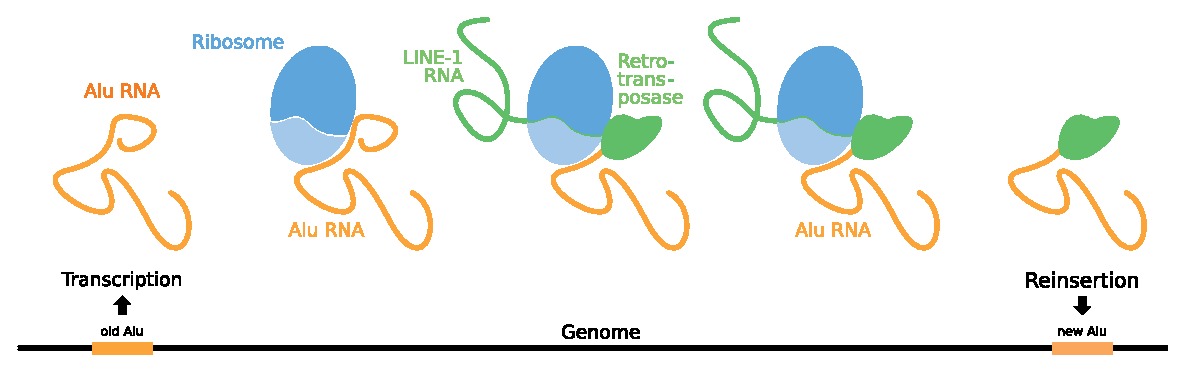
\includegraphics[width=\textwidth+\marginparwidth+\marginparsep]{
     04_GraphicFiles/02_alu_life.eps}}
\caption{Modification of figure 1a from \citet{Baar2022}, showing a schematic
  representation of Alu retrotransposition (left to right): the Alu element
  is transcribed -- the Alu RNA attaches itself to the exit tunnel of the
  ribosome through its SRP sequence homolog -- a LINE-1 RNA arrives at the
  ribosome and its retrotransposase is translated -- the Alu RNA hijacks the
  LINE-1 retrotransposase -- the LINE-1 retrotransposase reinserts the Alu
  element into a new genomic position.}
\label{fig:alulife}
\end{figure}

Alu elements, named after a restriction endonuclease of \textit{Athrobacter
luteus} which lead to their discovery, classified as short interspersed
nuclear elements (SINEs), are around \num{300}~bp long mobile DNA sequences
found in the human genome and other species
\citep{Schmid1975,Quentin1992,Lander2001,JO2007,Deininger2011}. They are RNA
retrotransposons, meaning that they are capable of copying themselves into new
positions in the genome. Due to this multiplication, Alu elements make up
\SI{11}{\percent} of the human genome by length, with more than \num{1}
million currently annotated loci \citep{Lander2001}.

The retrotransposition process of Alu elements shown in \cref{fig:alulife},
however, is error-prone and thus facilitates an Alu-specific sequence
evolution, giving rise to distinct Alu families from the old AluJ family over
AluS to the young AluY \citep{MR1991,Deininger1999,Batzer1996}. In general,
Alu elements are composed of a left arm and a right arm separated by a
variable A-rich region \citep{Evgenev2007}. The left arm contains an RNA
Polymerase III (Pol-III) promoter\label{sen:alupromo}, and the right arm holds
the UGU(NR) motif required for binding to the ribosome (see \cref{fig:alulife})
\citep{ Paolella1983,Dagan2004,A2012}. If Alu elements serve a function is,
so far, unknown. They can be harmful if a new insertion disrupts a gene or
other genomic region \citep{Deininger1999}. They have also been linked to
changes in transcriptional activity in general and under heat shock conditions
in particular \citep{Mariner2008,LL2017,Zhang2019}.

We wanted to address four questions regarding Alu elements, their
transcription, and their sequence features:

\begin{enumerate}[labelindent=0pt]
  \item Are Alu RNAs stable or unstable?\smallskip\newline
  Previous studies suggested that Alu RNAs should be less stable in the cell
  than regular mRNAs, meaning that they are degraded quickly \citep{An2004}.
  However, these results were obtained using only computational methods
  extrapolating from Alu sequence features and were not backed up by
  experimental data.\newline
  We could show that the distribution of Alu RNA half-lives predicted by our
  experimental approach is very similar to that of mRNAs, suggesting that Alu
  transcripts are more stable than previously thought.

  \item Are Alu elements transcribed primarily by Pol-III or by RNA
  Polymerase II (Pol-II), as well?\smallskip\newline
  While Alu elements do contain a Pol-III promoter sequence (see
  \cpageref{sen:alupromo}), it is surmised that Alu elements are not only
  transcribed by Pol-III but also, to a certain extent, by Pol-II
  \citep{Conti2015a,Zhang2019}. The experimental evidence for this is mostly
  indirect \citep{ Zhang2019,Panning1993,JAGADEESWARAN1981}. We have therefore
  conducted a Pol-II inhibition experiment and could show that Alu expression
  does indeed decrease under Pol-II inhibition, suggesting strongly that Alu
  transcripts arise, at least in part, directly from Pol-II activity.\newline
  This finding carries implications for differential expression analyses of
  the past. Often, Alu elements were used as a control group if Pol-II
  inhibition was performed, assuming wrongly that Alu transcription should be
  completely dependent on Pol-III \citep{Cordaux2009}.
  
  \item Is Alu transcription a side product of gene
  transcription?\smallskip\newline
  If a fraction of Alu transcription depends on Pol-II activity, a possible
  explanation could be that Alu elements are transcribed alongside regular
  genes \citep{Conti2015a,Zhang2019}. The results of our analyses weaken this
  hypothesis. While we cannot rule out that a fraction of Alu elements might
  be transcribed alongside genes, it is unlikely that this process contributes
  substantially to Alu expression.
  
  \item Is Alu expression influenced by sequence features?\smallskip\newline
  Previous studies unsuccessfully employed regular \textit{de novo} motif
  search to detect Alu sequence features that influence their expression
  \citep{Zhang2019}. We used two less common methods (see
  \nameref{subsubsec:aluanalysis}) and could uncover several influential
  positions and motifs that appear linked to changes in Alu expression.
  Additionally, some of the motifs match transcription factor binding profiles
  and may thus present promising targets for future investigations.
\end{enumerate}

\subsubsection{Methodology}\label{subsubsec:alumethod}
\addcontentsline{toc}{subsection}{Methodology}
This study made use of bulk, whole-genome RNA-seq data, partially generated
specifically for our investigation and partially repurposed from our earlier
publication \citet{Schwalb2016a}. The RNA was extracted from K562 cells, an
immortalised human suspension cell line of erythroleukemia cells
\citep{Andersson1979}. The sequencing data is noteworthy regarding two of its
characteristics:

Firstly, we used dynamic transcriptome analysis (DTA), specifically the 4sUseq
and the TT-seq methods \citep{Schwalb2012,Gressel2019}. DTA chemically labels
newly created transcripts, making them distinguishable from old RNAs still
present from before the labelling pulse. This allowed us to calculate the
ratio between old and new transcripts and thereby estimate these transcripts'
half-life.

Secondly, we performed a Pol-II inhibition experiment using \textalpha-%
amanitin, a toxic substance from the \textit{Amanita phalloides} fungus that
blocks Pol-II activity \citep{Lindell1970,Kedinger1970,Stirpe1967,Jacob1970}.
We treated K562 cells with \textalpha-amanitin and compared their RNA-seq data
with untreated samples. We could thus observe the effect of Pol-II inhibition
on different transcript classes, including Alu elements, \textit{bona fide}
Pol-II genes, and tRNAs, which are transcribed by the uninhibited Pol-III.

\subsubsection{Analysis}\label{subsubsec:aluanalysis}
\addcontentsline{toc}{subsection}{Analysis}

% ┌────────────────────────────────────────────────────────────────────────────┐
% │ 1. Are Alu RNAs stable or unstable?                                        │
% │    Half-Life Estimation                                                    │
% └────────────────────────────────────────────────────────────────────────────┘

Concerning\marginnote{Half-Life Estimation}\label{mar:alumle} the question,
if Alu RNAs are stable or unstable, we relied on the DTA data (see
\nameref{subsubsec:alumethod}), giving us two read counts for each Alu
element or gene, one from the labelled fraction and one from the total
fraction. With time, new labelled transcripts are created and old unlabelled
transcripts decay, meaning that the ratio of labelled RNAs increases until all
transcripts are labelled. Assuming exponential decay and steady-state
conditions, this ratio $r_{a}$ gives us the decay rate $\delta{}_{a}$ for any
Alu element or gene $a$ by
\begin{align*}
       r_{a} &= \nicefrac{l_{a}}{t_{a}}=1-\exp(-\delta_{a}\Delta t)
\\ \ln r_{a} &= \ln\left(1-\exp(-\delta_{a}\Delta t)\right)
\end{align*}
where $l_{a}$ and $t_{a}$ are the numbers of labelled or total RNA molecules
and $\Delta{}t$ is the labelling pulse’s duration, meaning the time that
passed after the labelling agent was added and before the RNA sequencing was
performed. From the decay rate $\delta{}_{a}$ the half-life
$t_{\nicefrac{1}{2},a}$ is given by
\begin{align*}
t_{\nicefrac{1}{2},a}=\frac{\ln\left(2\right)}{\delta_{a}}
\end{align*}
To estimate the ratio between labelled and total RNA molecules from the
measured reads, we used maximum likelihood estimation (MLE) \citep{Rossi2018}
(see also \nameref{sec:methoverview}). We made several assumptions to simplify
the estimation, owing to the general paucity of Alu read counts caused by
their low expression. We assume steady-state conditions, use a Poisson
distribution to model read counts instead of a zero-inflated negative binomial
distribution, and neglect non-constant labelling efficiencies for short
labelling periods. This means that our estimation can only serve as an
assessment to compare the relative half-life distributions of Alu elements and
genes. Its predictions do not represent explicit half-life values. Still, the
very similar distribution of Alu and gene half-lives suggests that the
stability of Alu transcripts is greater than would be expected from sequence
features alone.
\bigbreak

\begin{figure}[b!]
\centering
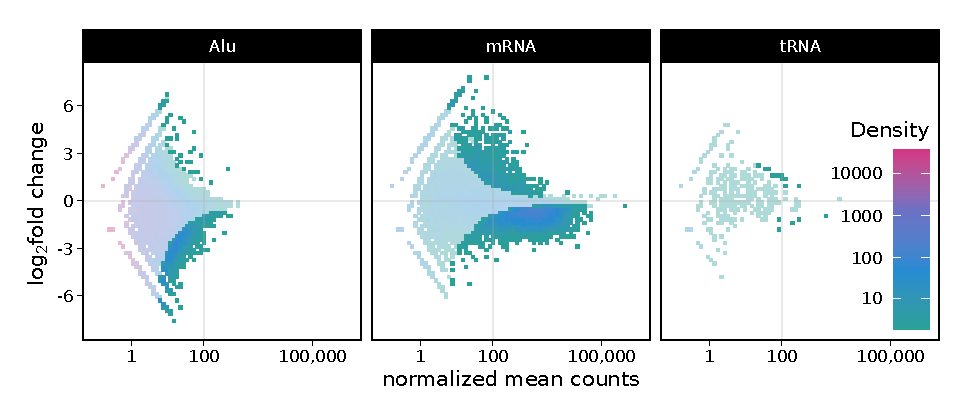
\includegraphics[width=\textwidth]{04_GraphicFiles/02_alu_deseq2.eps}
\caption{Modification of figure 3e from \citet{Baar2022}. 2D density heatmap
  showing the DESeq2 differential expression of Alu elements, mRNAs, and tRNAs
  under \textalpha-amanitin Pol-II inhibition. Semi-transparent areas do not
  pass the significance threshold. Loci with a normalised mean expression
  below 0.1 are excluded, with affects \SI{51}{\percent} of all annotated
  Alu loci and practically no mRNAs or tRNAs.}
\label{fig:aludeseq2}
\end{figure}

\noindent The \textalpha-amanitin\marginnote{Differential Expression Analysis}
\label{mar:aludeseq2} Pol-II inhibition experiment was the key to
investigating the origin of Alu transcripts. To analyse the RNAseq
measurements, we used the DESeq2 package for R \citep{Love2014}. The standard
assumption of DESeq2's internal normalisation strategy is that there are no
substantial, systematic global expression changes between samples. Due to the
inhibition of Pol-II, we have to assume that this does not hold. We,
therefore, used mitochondrial transcripts (mtRNAs) for normalisation, which
are unaffected by the \textalpha-amanitin treatment. This is because the
mitochondrial polymerase that transcribes mtRNAs is not inhibited by
\textalpha-amanitin \citep{Menon1971,Reid2830,Saccone1971}. The resulting
differential expression estimates of Alu elements, mRNAs, and tRNAs, which we
used as a negative control as they are transcribed by Pol-III, which is also
unaffected by \textalpha-amanitin, are shown in \cref{fig:aludeseq2}
\citep{ White1997}. As expected, tRNAs remain largely unaffected by the
\textalpha-amanitin treatment, while mRNAs exhibit downregulation. Notably,
Alu RNAs also appear downregulated under Pol-II inhibition, suggesting
strongly that Alu elements are, at least to a certain extent, transcribed by
Pol-II.
\bigbreak

\noindent To address\marginnote{Correlation Analysis}\label{mar:alucor} the
follow-up question if the apparent expression of Alu elements by Pol-II may
result from Alu RNAs being side products of gene transcription, we argued as
follows \citep{Conti2015a,Zhang2019}: If Alu elements were transcribed
alongside genes, those inside or close to genes should show higher expression
compared to Alu elements that are far away from genes. The expression of a
gene should also correlate with the expression of Alu elements inside or close
to it. Finally, Alu elements should show a bias towards lying in sense
direction with regard to their associated gene.
\pagebreak

% page break ...................................................................

\noindent
While we did detect a significantly higher expression of Alu elements that lie
inside or close to genes, this effect can result easily from increased genome
accessibility in areas of active gene transcription \citep{Guo2016}. This also
biases the correlation analysis. Therefore, we examined the difference in
correlation strength between Alu element and gene transcription if split by
sense and antisense Alu direction. As we detected no difference in correlation
strength and also found that Alu elements show no preference for inserting
themselves in sense direction into genes, we conclude that it is unlikely that
Alu transcription is a side product of gene transcription. While our results
do not rule out that some Alu transcripts are created alongside genes, this
does not appear to be a major source for Alu RNAs.
\bigbreak

\noindent To search\marginnote{Generalised\\ Linear Model}\label{mar:aluglm}
for sequence features that influence Alu expression, we pursued two different
approaches. Firstly, to analyse Alu elements on a per-base level, we used a
generalised linear model created with the glmnet package for R
\citep{Nelder1972, Friedman2010} (see also \nameref{sec:methoverview}). We
assumed a Poisson family distribution response type and used an elastic mixing
parameter \textalpha{} of \num{1} (full Lasso penalty, no ridge regression
penalty), no fitted intercept parameter, and \num{1000}$\times$ cross-%
validation. To create the input matrices, we aligned all Alu sequences against
the Alu consensus sequence and encoded base exchanges, deletions, and
insertions for each position as a binary matrix. For these three types of
point mutation, we trained GLMs with the Alu read counts as a response
variable. Finally, we used the Euclidean norm of the three obtained effect
sizes for each position in the Alu consensus sequence to judge their
respective importance, uncovering several influential positions.
\bigbreak

\noindent Secondly,\marginnote{De Bruijn Graph}\label{mar:alugraph} to detect
larger sequence features, we created a De Bruijn graph of all Alu sequences
using bifrost v1.0.5 \citep{Holley2020}. A De Bruijn genome graph is a way to
encode sequence variability in a graph structure \citep{Chikhi2014}. This
method is based on general De Bruijn graphs, which are directed graphs
representing the overlap between symbol strings
\citep{Sainte-Marie1894,DeBruijn1946,Good1946}. In the context of biological
data, the strings are sequences of length $k$ (k-mers), using DNA or RNA bases
as symbols. Each node in the graph represents one unique k-mer present in the
source data from which the k-mers are generated. Each node also represents its
own reverse complement, depending on the direction in which it is traversed.
Edges in the graph represent overlaps. For example, a sequence $S_{1}$ would
be connected by an edge to another sequence $S_{2}$ if they overlap except for
one base, such that
\begin{align*}
S_{1}=\left(s_{1},s_{2},\ldots,s_{n}\right)
  \quad\text{and}\quad
  S_{2}=\left(s_{2},s_{3},\ldots,s_{n},s_{n+1}\right)
\end{align*}
With \num{4} biological bases, each node can have up to \num{16} edges
connected to it, \num{4} in- and \num{4} out-edged in forward direction and
again in reverse complement direction. If a graph is compacted, sequential
nodes without branching edges can be combined into a single node representing
a sequence with a length greater than $k$.

As the De Bruijn genome graph we constructed from all Alu sequences was almost
complete with an in-degree per node of \num{>7.99}, we focused on the
constituent k-mers and disregarded the graph structure in downstream analyses.
We filtered the k-mers using two criteria. The expression of Alu elements
possessing the k-mer needed to be significantly different from those not
possessing it. Also, we took each k-mers's suffix and prefix into account.

Assuming a k-mer with the structure $\text{X\,J\,Y}$, with
$\text{X},\text{Y}\in\{A,C,T,G\}$ and $\text{J}$ a fixed 2-mer, to assure that
$\text{X\,J\,Y}$ is causal for observed changes in Alu transcription, we test
the group of Alu elements containing $\text{X\,J\,Y}$ against the group
containing the k-mer's prefix $\text{X\,J}$ or its suffix $\text{J\,Y}$, but
not the full k-mer. Thus we can be confident that the observed effect is
caused by the complete k-mer and not just its partial sequence.

With this method. we uncovered several statistically significant and
biologically relevant sequence motifs which previous attempts using regular
\textit{de novo} motif search did not \citep{Zhang2019}.
\bigbreak

\noindent In summary, we found that Alu transcripts appear to be as stable as
mRNAs, more stable than previously thought. In addition, we found evidence for
Alu elements originating in independent Pol-II transcription, not originating
as side products of gene transcription. Finally, we also identified a list of
sequence features that influence Alu expression and might therefore be
promising targets for future investigations.
\pagebreak

% page break ...................................................................

\null
\vfill
\noindent My contribution to this publication was the complete bioinformatic
and statistical analysis.\nopagebreak
\medskip
\begin{tcolorbox}[
  boxrule=0pt, leftrule=1pt, colframe=s-blue, colback=white, sharp corners=all]%
  \raggedright
  Baar, T., Dümcke, S., Gressel, S., Schwalb, B.,
  Dilthey, A., Cramer, P., Tresch, A. (2022).
  
  \smallskip
  \href{https://doi.org/10.1093/g3journal/jkac054}
    {RNA transcription and degradation of Alu retrotransposons depends on
    sequence features and evolutionary history}

  \smallskip
  \textit{G3: Genes}\thinspace{}|\thinspace{}\textit{Genomes}%
    \thinspace{}|\thinspace{}\textit{Genetics, 2160-1836}
\end{tcolorbox}

% ┌────────────────────────────────────────────────────────────────────────────┐
% │ PDF                                                                        │
% └────────────────────────────────────────────────────────────────────────────┘

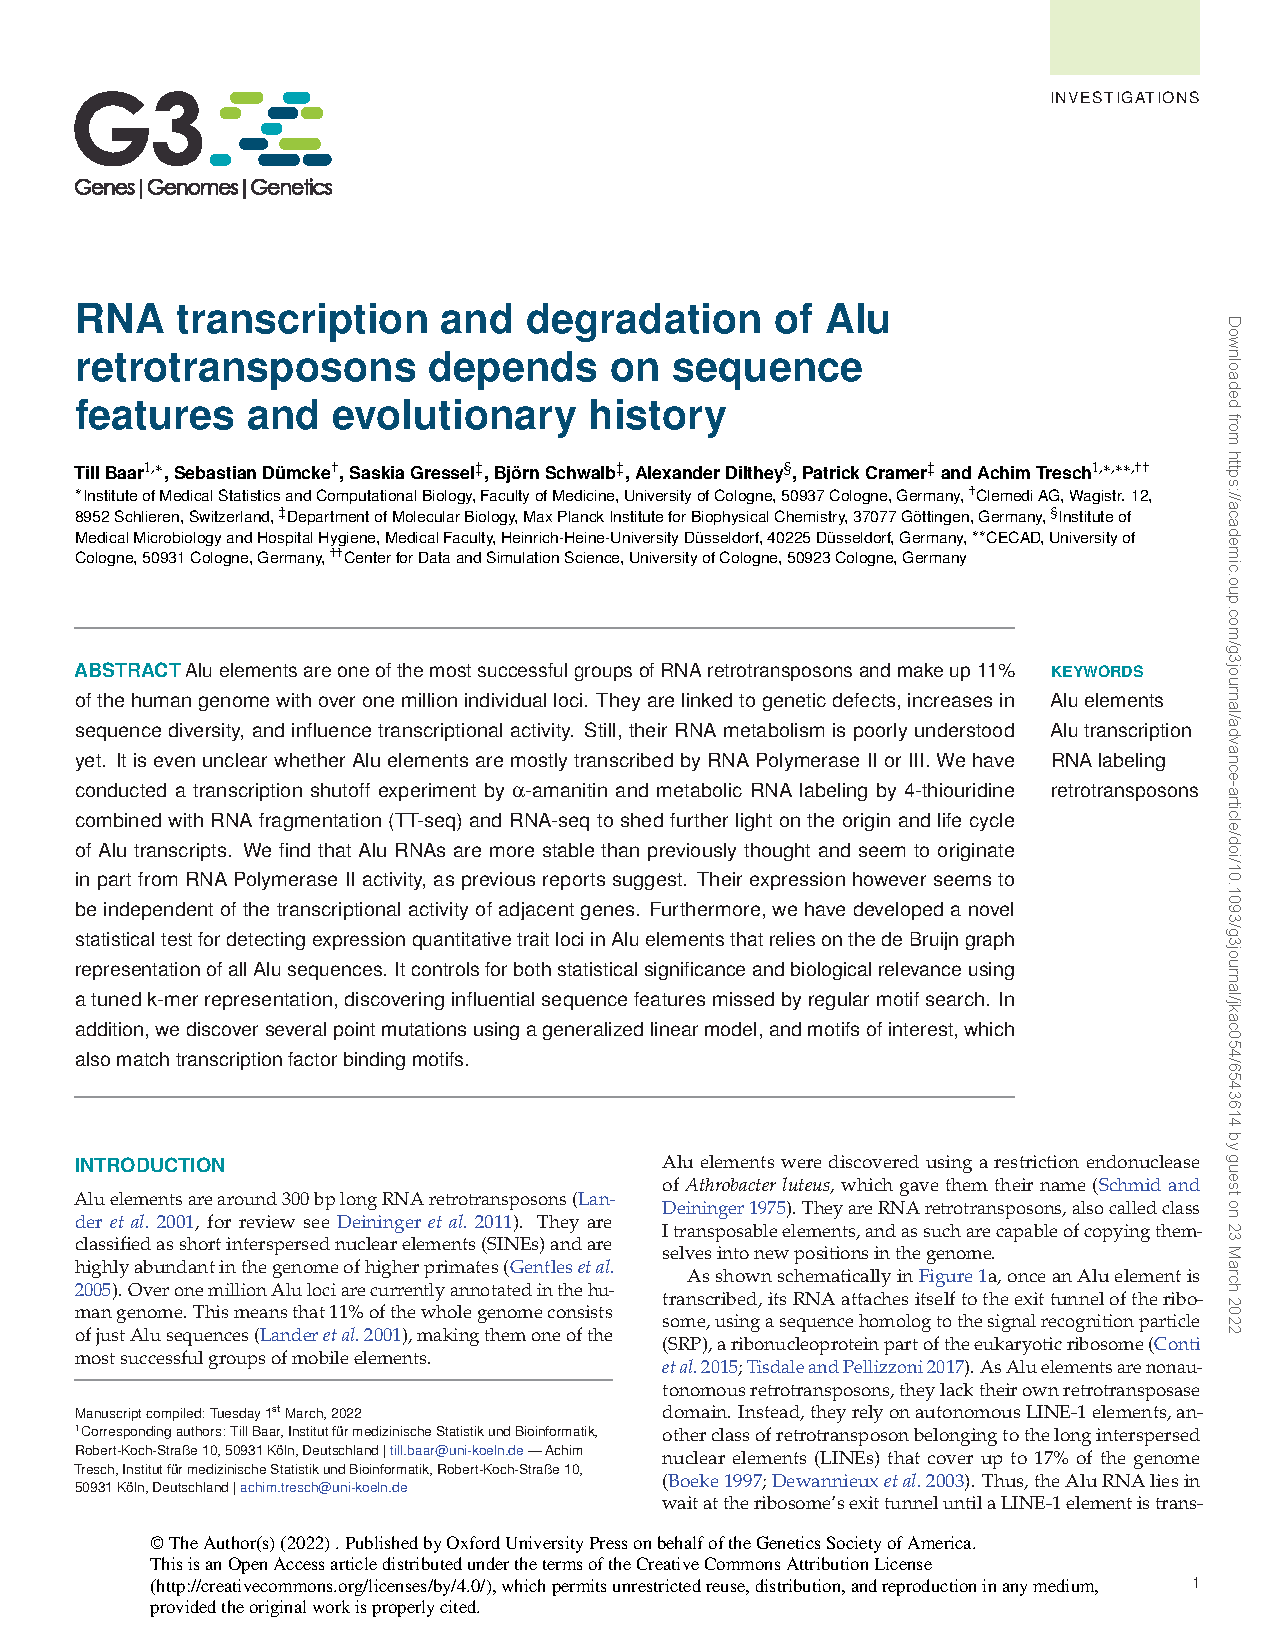
\includepdf[pages=-, addtotoc={1, section, 1,
  RNA transcription and degradation of Alu retrotransposons depends on
  sequence features and evolutionary history,
  RNA transcription and degradation of Alu retrotransposons depends on
  sequence features and evolutionary history}]
  {"07_Publications/Baar2022.pdf"}
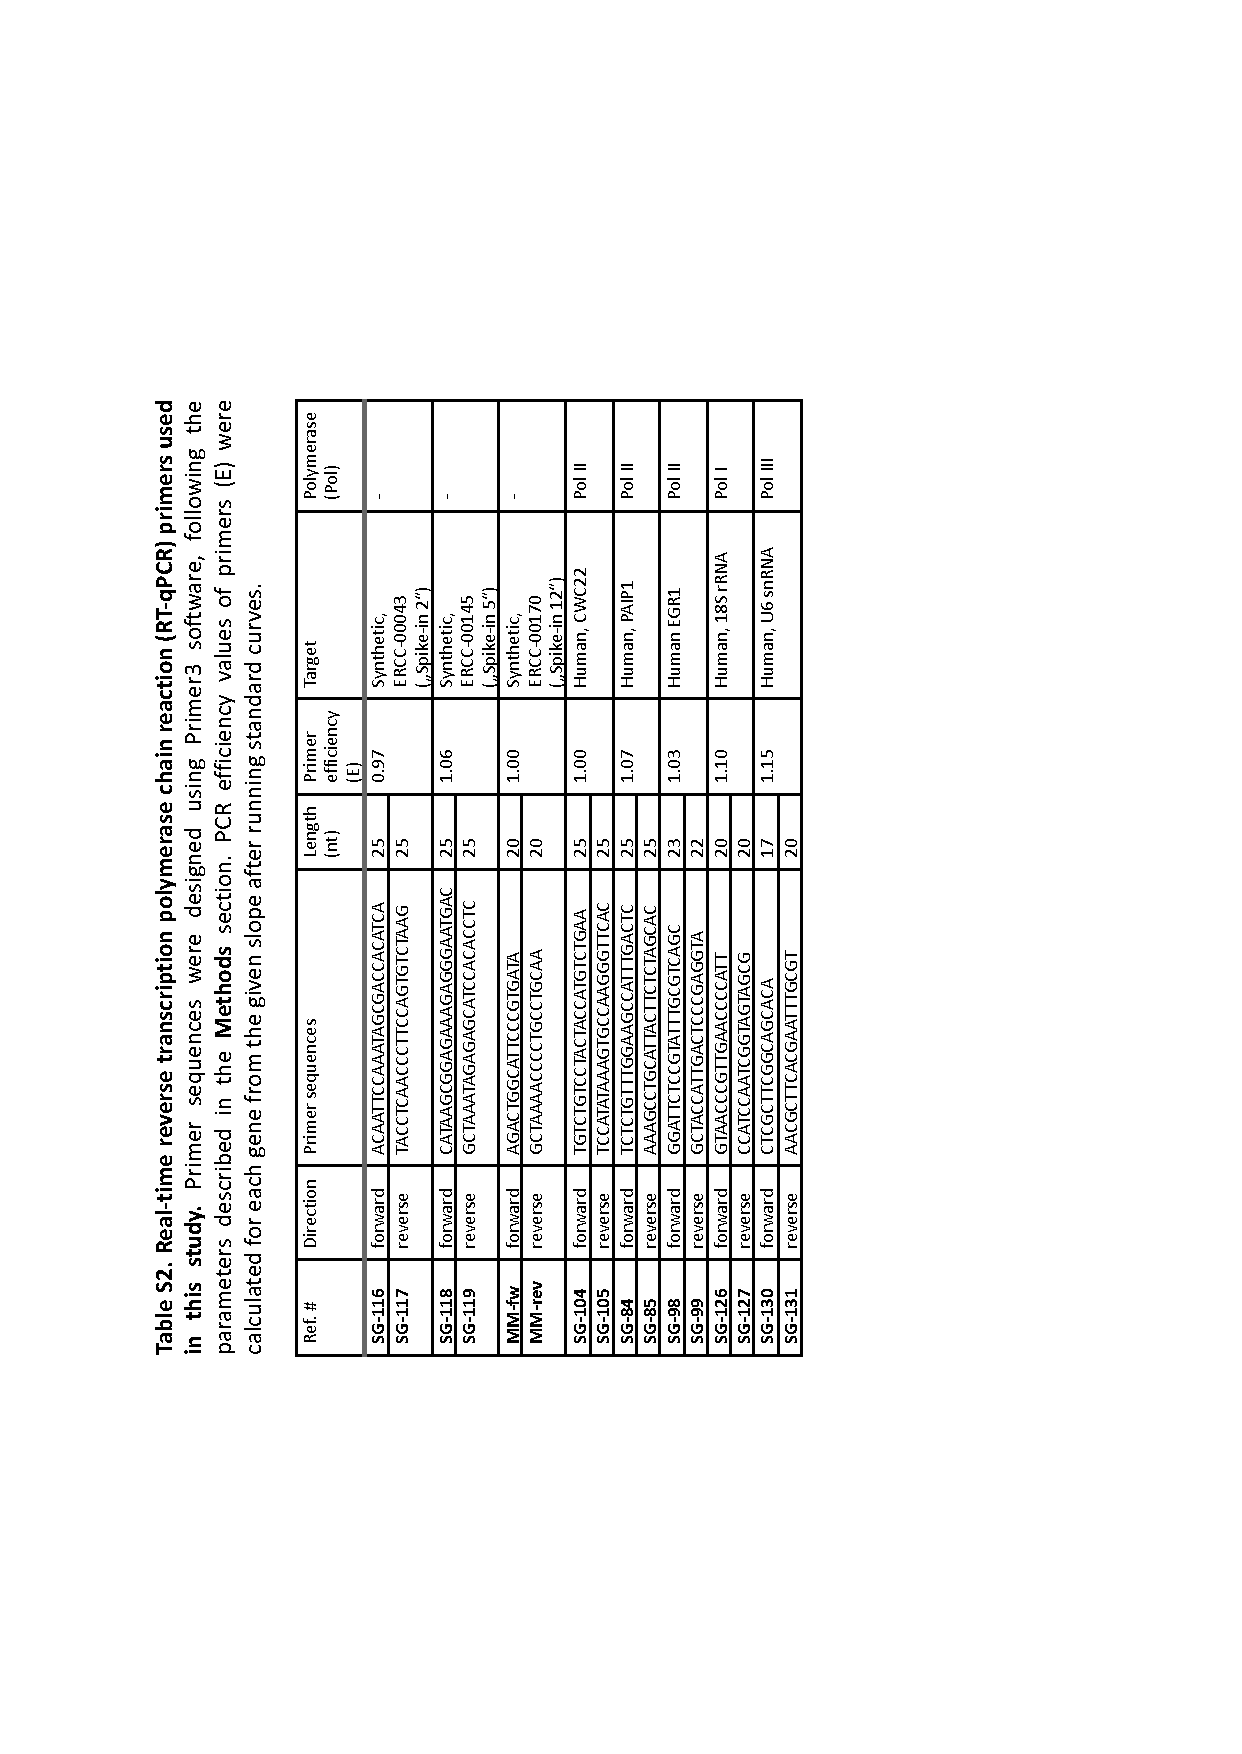
\includepdf[pages=-]{"07_Publications/Baar2022sup.pdf"}

\null
\thispagestyle{empty}
\newpage
% ┌────────────────────────────────────────────────────────────────────────────┐
% │ ANGIO PAPER                                                                │
% │   Endoscopic hemostasis makes the difference: Angiographic treatment in    │
% │   patients with lower gastrointestinal bleeding                            │
% └────────────────────────────────────────────────────────────────────────────┘

\chapter{Angiography for Gastrointestinal Bleeding}
\sectionmark{Angiography for Gastrointestinal Bleeding}

This retrospective study's goal was the identification of variables that
increase the chance for a patient suffering from lower gastrointestinal
bleeding (LGIB) to benefit from angiography.

LGIB describes any form of gastrointestinal (GI) bleeding occurring in the
lower gastrointestinal tract, which includes most of the small intestine and
all of the large intestine \citep{Treuting2018}. GI bleeding can have many
causes, including cancer, and the resulting blood loss can lead to shock,
syncope, and even death with a chance of around \SI{15}{\percent} \citep{%
Rockey2005,PrasadKerlin2013,Wang2013,Kim2014}. While the majority of GI
bleedings subside on their own or can be arrested through endoscopic
treatment, endoscopy cannot detect the cause of LGIB in \SI{40}{\percent} of
all cases \citep{Yamada2015,Werner2018}. Once localised, though, over \SI{90}{%
\percent} of LGIBs can be treated successfully. It is therefore vital that
in cases with symptoms severe enough to result in hospitalisation, the source
of bleeding is identified quickly and reliably and that hemostasis is
achieved, be that through endoscopic treatment or surgery \citep{Strate2010,
Werner2018}.

It is at this point that angiography comes into the picture. Angiography is a
medical radiological imaging technique that visualises blood vessels, as well
as bleeding. This is achieved by injecting a radio-opaque contrast agent into
the bloodstream in conjunction with X-ray imaging \citep{Martin2015}. Catheter
angiography (CA), coupled with transarterial embolisation (TAE), a method to
stop the flow of blood to a selected area of tissue, has high technical
success rates of \SIrange{90}{100}{\percent} and low complication rates of
\SIrange{1}{5}{\percent} \citep{Tan2008,Evangelista2000,Strate2010,Kim2017,
Lee2018,Oakland2019,Pannatier2019}. However, it also exposes the patient to
the  contrast agent and X-ray imaging, while endoscopy requires only
anaesthesia. Angiography is also a more complex technique and involves the
patient's referral to a radiologist. Thus, the decision of when to conclude
endoscopic procedures and begin angiographic treatment is challenging. If
angiography is initiated too late, the patient is subjected to multiple
failed endoscopies, while if angiography is used too early, the patient is
needlessly exposed to the side effects of radiological treatment.

Accordingly, our goal was to construct a decision-making aid for clinicians,
assisting them in deciding when to apply endoscopy and when to apply
angiography to treat LGIB. While prospective investigations will be required
to consolidate our results, the predictors we selected may contribute to the
development of future official guidelines.

\subsubsection{Methodology}\label{subsubsec:angiomethod}
\addcontentsline{toc}{subsection}{Methodology}
The data for this study was collected over the span of \num{11} years at a
maximum care hospital and included \num{133} patients. Of these, the treatment
group consisted of \num{41} patients that received CA for LGIB, while the
control group of \num{92} patients was treated for LGIB without angiography.
\num{110} variables were recorded for each patient, of which \num{20} were
designated as being of particular clinical relevance according to expert
opinion.

As the data collection period was so extensive and involved many clinicians,
no precise statements concerning the methods used for data recording can be
made. The data types were also highly diverse, ranging from binary labels,
such as clinical success, time intervals and ordinal variables, to numeric
laboratory test results.

\subsubsection{Analysis}\label{subsubsec:angioanalysis}
\addcontentsline{toc}{subsection}{Analysis}
All of our data was ultimately recorded by humans and was thus flawed, which
may sound harsh but is true more often than not. Therefore, data cleaning and
validation was the first step, an arduous step that is nonetheless crucial.

Descriptive statistics followed, along with na\"{i}ve pairwise correlation
analyses between selected variables and nonparametric tests, using either
Fisher's exact test or the Mann-Whitney U test, depending on the data at hand
\citep{Winters2010} (see also \nameref{sec:methoverview}). Then, as no biases
or other incongruities arose, the principal analysis could commence.

Two items had to be considered at the start. Firstly, we had to establish that
we assume the professional decision of the clinicians to treat a patient
either with or without angiography to be founded in their medical expertise.
The alternative assumption would be that we cannot equate a patient receiving
angiographic treatment with the need of a patient to receive such treatment.
Under this alternative assumption, our investigation could not have drawn any
meaningful conclusions. It is a natural limitation of a retrospective study,
which is also why prospective investigations are necessary before an official
guideline can be established. Hence, we assume that a causal link exists
between a patient's statistics and treatment.

\begin{figure}[b!]
\centering
 \makebox[\textwidth][l]{
   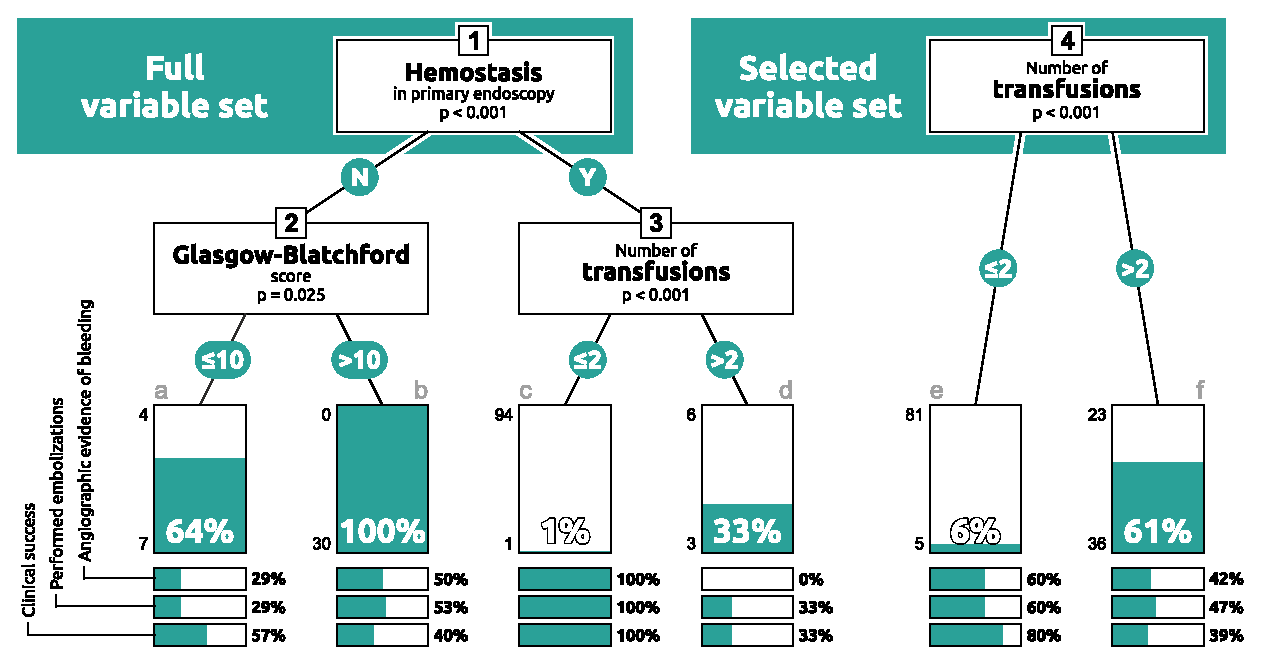
\includegraphics[width=\textwidth+\marginparwidth+\marginparsep]{
     04_GraphicFiles/03_angio_trees.eps}}
\caption{Modification of figures 2 and 3 from \citet{Werner2021}. Conditional
  inference trees were constructed from either the complete data set (left) or 
  a set of variables selected for clinical relevance (right). Each binary 
  split (numbered boxes 1 to 4) is annotated with its p-value. Each terminal 
  node (vertical bars a to f) shows the percentage of angiography-positive 
  cases.}
\label{fig:angiotree}
\end{figure}

Secondly, our goal was to create a decision-making aid for clinicians, helping
them decide when to switch from endoscopy to angiography for the treatment of
LGIB. While we could have constructed a complex regression model to predict
the method suitable for a patient as best as possible, such a model would not
be applicable in the daily clinic routine. While computer-based predictors to
guide treatment decisions may become mundane in the future, this is not yet
the case. Consequently, our decision-making aid needed to be easily traceable,
allowing the clinician to arrive at a prognosis by following a transparent
algorithm. Accepting that, in consequence, our final model may be undercomplex
to some extent and thus prone to underfitting, we elected to use conditional
inference trees (see \nameref{sec:methoverview}).

\begin{figure}[b!]
\centering
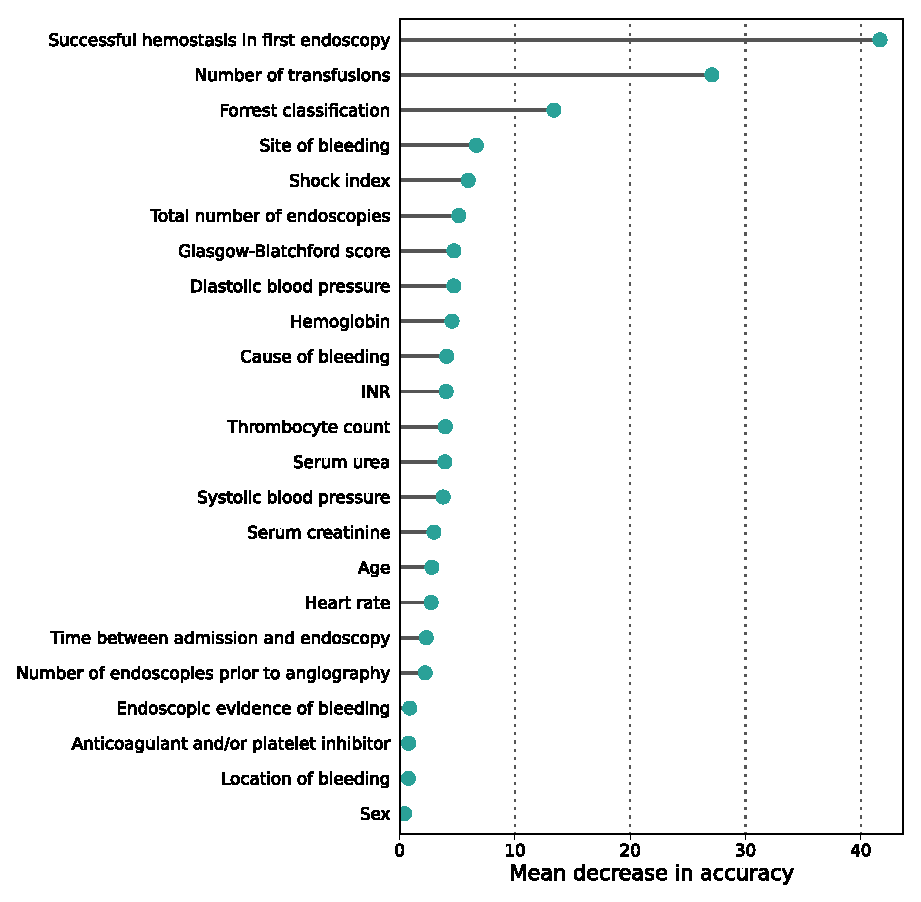
\includegraphics[width=\textwidth]{04_GraphicFiles/03_angio_forest.eps}
\caption{Modification of figure 1 from \citet{Werner2021}. Variable importance
  in terms of mean decrease in accuracy of the features included in the   
  construction of the decision trees computed using a random forest
  classifier with \num{10000} trees and \num{25} iterations.}
\label{fig:angioforest}
\end{figure}

\noindent We decided to construct two decision trees shown in \cref{%
fig:angiotree}, one based on all recorded patient variables and another based
solely on the clinically relevant variables. The trees offer a straightforward
way for a clinician to determine if a patient should receive angiography or
not. Using the tree based on the full variable set as an example, only two
queries are needed for a patient: If hemostasis was achieved in the first
endoscopy, the number of blood transfusions a patient has received is needed.
On the other hand, if the primary endoscopy failed to achieve hemostasis, the
Glasgow-Blatchford Bleeding Score (GBS) of the patient becomes the telling
factor. The GBS is used to classify the severity of GI bleeding \citep{%
Laursen2015}.

In addition, we also used random forest to compute the mean decrease in
accuracy variable importance measure for the variables used in constructing
the decision trees \citep{Han2016} (see also \nameref{sec:methoverview}). This
was done to substantiate the variable choices made by the decision tree
models. Mean decrease in accuracy is computed by permuting the out-of-bag (OOB)
data, referring to the data not included in an individual bootstrap sample.
The error rate on the OOB data is computed once and computed again after
permuting each predictor variable.  The difference between the two is averaged
over all bootstrap samples and normalised by the standard deviation of the
differences. The resulting variable importance is a positive value that
increases the more influential any given variable is. The results agreed
satisfactorily with the decision trees, with the success of achieving
hemostasis in the primary endoscopy (binary split 1 in \cref{fig:angiotree})
and the number of transfusions (binary splits 3 and 4 in \cref{fig:angiotree})
being the two most important variables.

\vfill
\noindent My contribution to this publication was the complete bioinformatic
and statistical analysis.\nopagebreak
\medskip
\begin{tcolorbox}[
  boxrule=0pt, leftrule=1pt, colframe=s-blue, colback=white, sharp corners=all]%
  \raggedright
  Werner, DJ., Baar, T., Kiesslich, R., Wenzel, N., Abusalim, N., Tresch, A.,
  Rey, JW. (2021).
  
  \smallskip
  \href{https://www.wjgnet.com/1948-5190/full/v13/i7/221.htm}
    {Endoscopic hemostasis makes the difference: Angiographic treatment in
    patients with lower gastrointestinal bleeding}

  \smallskip
  \textit{World J Gastrointest Endosc, 13(7): 221-232}
\end{tcolorbox}

% ┌────────────────────────────────────────────────────────────────────────────┐
% │ PDF                                                                        │
% └────────────────────────────────────────────────────────────────────────────┘

\includepdf[pages={4-15}, addtotoc={4, section, 1,
  Endoscopic hemostasis makes the difference: Angiographic treatment in
  patients with lower gastrointestinal bleeding,
  Endoscopic hemostasis makes the difference: Angiographic treatment in
  patients with lower gastrointestinal bleeding}]
  {"99_Publications/Werner2021.pdf"}

\null
\thispagestyle{empty}
\newpage
% ┌────────────────────────────────────────────────────────────────────────────┐
% │ NANOSTRING PAPER                                                           │
% │   Genetic instability and recurrent MYC amplification in ALK-translocated  │
% │   NSCLC: a central role of TP53 mutations                                  │
% └────────────────────────────────────────────────────────────────────────────┘

\chapter{Theragnosis Biomarkers in Lung Cancer}
\sectionmark{Theragnosis Biomarkers in Lung Cancer}

This study investigates the connection between rearrangement of the anaplastic
lymphoma kinase (\textit{ALK}) and \textit{TP53} mutations in human non-small
cell lung cancer.

Lung cancer, one of the main causes of death in humans \citep{Siegel2018}, is
traditionally divided into two types: small cell lung cancer (SCLC) and non-%
small cell lung cancer (NSCLC), which constitutes over \SI{80}{\percent} of
all cases \citep{Reck2014}. However, NSCLC has proven to be too diverse and is
now treated as a collection of many different cancer types that each require
individual treatment regimes \citep{Boolell2015}. One of these is \textit{ALK+}
lung cancer, in which the \textit{ALK} gene breaks and fuses with other genes
\citep{Holla2017}.

The \textit{ALK} gene encodes a receptor tyrosine kinase that is only expressed
in early embryonic development and is involved in cell proliferation, survival,
and differentiation of the nervous system \citep{Iwahara1997}.
% While the ligands of ALK are unknown, its downstream signalling pathways have
% been characterised \citep{Stoica2001,Stoica2002,Bennasroune2010,Murray2015}.
However, in \textit{ALK+} lung cancer, the fusion of \textit{ALK} to other genes
causes uncontrolled activation of its downstream signalling paths through the
fusion partner's promoter \citep{Holla2017}. In turn, tyrosine kinase inhibitors
(TKI) have been shown to be an effective treatment for \textit{ALK+} lung cancer
\citep{Kwak2010,Reck2014}.

\citet{Gainor2016} found that \SI{33}{\percent} of \textit{ALK+} tumours also
show mutations in the \textit{TP53} gene, and \citet{Aisner2018} discovered
that \textit{TP53} mutations reduced patient survival in \textit{ALK+} lung
cancer. \textit{TP53} is classified as a tumour suppressor gene, as it
prevents genome mutation \citep{Surget2013}. It plays a role in cell cycle
regulation and apoptosis, activating DNA repair mechanisms when damage has
been sustained and halting the cell cycle until the damage is repaired. If the
damage is too severe and cannot be repaired, it initiates programmed cell
death. \textit{TP53} mutations are thus frequent in many cancer types, as
inactivation of \textit{TP53} severely compromises tumour suppression \citep{%
Olivier2010}.

Our assumption, which we could corroborate in the publication, was that
mutations in \textit{TP53} lead to genetic instability, which in turn promote
the development of resistance mechanisms, reducing patient survival rate in
\textit{ALK+} lung cancer \citep{Alidousty2018}.

% \bigbreak
% \noindent

\subsubsection{Methodology}\label{subsubsec:alkmethod}
\addcontentsline{toc}{subsection}{Methodology}
To show that \textit{ALK+} lung cancers with \textit{TP53} mutations do
exhibit genetic instability, we examined tumour tissue samples from a total of
\num{423} patients originating in routine molecular diagnostics. However,
depending on the used laboratory procedure, not all samples were eligible for
analysis.

Bulk, panel-based DNAseq was used to categorise the tumour samples according
to the variants present in a set of genes of interest. In panel-based
sequencing, a mix of PCR primers limits the analysis to selected genomic
target loci. This has the benefit of increasing the coverage of these loci, as
the vast majority of generated reads is focused on the panel regions. As this
method could not detect large-scale genomic rearrangements, like the \textit{%
ALK} translocation, it was paired with fluorescence \textit{in situ}
hybridisation (FISH). In this technique, fixed tumour tissue sections are
treated with fluorescent molecular probes. The probes target multiple parts of
a gene of interest, \textit{ALK}, in this case, hybridising to the sequence's
position on the respective chromosome in the nucleus. The tissue sections are
then analysed under a microscope. If no rearrangement has taken place, the
probes show up as a single fluorescent spot in the nucleus. However, if parts
of the \textit{ALK} gene have fused to another gene on another chromosome,
multiple spots become visible, as can be seen in figure 2 of the included
publication. FISH offers the benefit of being a well- established laboratory
technique in cancer diagnostics, reliable at detecting translocation events
with clinical relevance. Its shortcomings are that is it a labour-intensive
protocol and can only detect specific breakpoints, which is why FISH will most
likely be replaced by genome-wide DNAseq in the future \citep{Skovgaard2011}.
Finally, immunohistochemistry (IHC) antibody staining was used to detect the
presence of the TP53 protein in the tissue samples. As \textit{TP53} is only
active in early embryonic development, its presence in tumour cells indicates
aberrant \textit{TP53} expression.

A fraction\marginnote{Nanostring}\label{mar:nanostring} of the tissue samples
were also analysed using the NanoString nCounter platform \citep{%
Geiss2008,Tsang2017}, as described in \citet{Kim2016}. This technology uses
fluorescent probes to generate direct counts of DNA molecules in tissue
samples. First, a mixture of probes is added to the extracted DNA. Each probe
targets a specific sequence unique to a gene of interest so that each molecule
containing that sequence is hybridised to a probe. The probes carry unique
fluorescent barcodes composed of six spots, each spot being one of four
colours. The barcodes are read by the instrument through automated fluorescent
microscopy and counted, generating raw counts that report the physical number
of DNA molecules containing the sequence of interest on the instrument's
slide. This technique has several advantages over sequencing-based
technologies, mostly its robustness with regard to fixed samples and the
reproducibility of its count data, as no amplification bias is introduced.
However, like in panel-based DNA sequencing, the genes that can be analysed
are limited by the used probes, of which there are no more than \num{800} per
panel (assuming that each spot needs to be a different colour from its
predecessor leaves $4\cdot3^{\,5}\!=972$ possible barcodes, of which some are
needed for quality control and normalisation purposes).

\begin{figure}[b!]
\centering
\includegraphics[width=\textwidth]{04_GraphicFiles/04_molpatho.eps}
\caption{Modification of figure 1c from \citet{Alidousty2018}. Copy number
  plots of \textit{ALK+} cell lines harbouring wild type \textit{TP53} (middle
  and right facet) or mutated \textit{TP53} (left facet). Copy numbers of
  \num{87} genes were determined by NanoString nCounter technology (see
  \nameref{mar:nanostring}). Alternating colours denote chromosome boundaries.}
\label{fig:molpatho}
\end{figure}

Finally\marginnote{Cell Culture}\label{mar:cellcult}, the results obtained
from the tumour tissue samples were furthermore supplemented by analysing
three different \textit{ALK+} human lung cancer cell lines with different
\textit{TP53} statuses. Using cell culture samples has the benefit that no
fixation procedure is applied and that the amount of available genetic
material is unlimited for all practical concerns. This allowed for a chromatin
immunoprecipitation DNA sequencing (ChIPseq) analysis to be performed on the
cell culture samples. ChIPseq limits bulk DNAseq to regions of the genome
bound by specific proteins \citep{Park2009}. First, proteins bound to the
genome are chemically immobilised to prevent detachment, and the DNA is
fragmented. Then, antibodies are used to pull out only those DNA fragments
bound by specific proteins. Finally, these fragments are sequenced and mapped
to the genome. In our study, we used ChIPseq to ascertain the binding of MYC
\citep{Dang2012}, a transcription factor that, if overexpressed due to
increased \textit{MYC} copy numbers, grants \textit{ALK+ TP53}-mutated tumour
cells a proliferative advantage over their wild-type counterpart. We could
observe this by monitoring the growth of cell cultures in which we induced
transient \textit{MYC} overexpression.

\subsubsection{Analysis}\label{subsubsec:alkanalysis}
\addcontentsline{toc}{subsection}{Analysis}
Of the three publications included in this dissertation, this is the one with
the most straightforward analysis. The central question was if \textit{ALK+}
tumour cells with a \textit{TP53} mutation show higher genetic instability
than those without. Genetic instability, in this case, was defined as higher
variability in the copy number of genes. In diploid organisms like humans,
autosomal genes have two copies each, one for each chromosome \citep{Hartl2009}.
Every deviation from a copy number of \num{2} can thus be seen as a copy
number alteration.

In this case, the choice of laboratory protocol simplified the analysis. As
NanoString nCounter technology was employed (see \nameref{mar:nanostring}),
the data sets consisted of count matrices giving the number of fluorescent
probe detections, automatically normalised between samples through internal
controls. Without a prior PRC reaction, no amplification biases could be
introduced. We thus chose to use the Brown-Forsythe test for the equality of
variances \citep{Brown1974} (see also \nameref{sec:methoverview}), which
confirmed the apparent increased genetic instability of \textit{ALK+ TP53}-
mutated cells, as exemplified in \cref{fig:molpatho}.

\enlargethispage{\baselineskip}

\vfill
\noindent My contribution to this publication's bioinformatic and statistical
analysis part was the copy number analysis, which facilitates the study's
central finding.\nopagebreak
\medskip
\begin{tcolorbox}[
  boxrule=0pt, leftrule=1pt, colframe=s-blue, colback=white, sharp corners=all]%
  \raggedright
  Alidousty, C., Baar, T., Martelotto, L. G., Heydt, C., Wagener, S.,
  Fassunke, J., Duerbaum, N., Scheel, A. H., Frank, S., Holz, B., Binot, E.,
  Kron, A., Merkelbach-Bruse, S., Ihle, M. A., Wolf, J., Buettner, R.,
  Schultheis, A. M. (2018).
  
  \smallskip
  \href{http://doi.wiley.com/10.1002/path.5110}
    {Genetic instability and recurrent MYC amplification in ALK-translocated
    NSCLC; a central role of TP53 mutations}

  \smallskip
  \textit{J Pathol (July):67–76.}
\end{tcolorbox}

% ┌────────────────────────────────────────────────────────────────────────────┐
% │ PDF                                                                        │
% └────────────────────────────────────────────────────────────────────────────┘

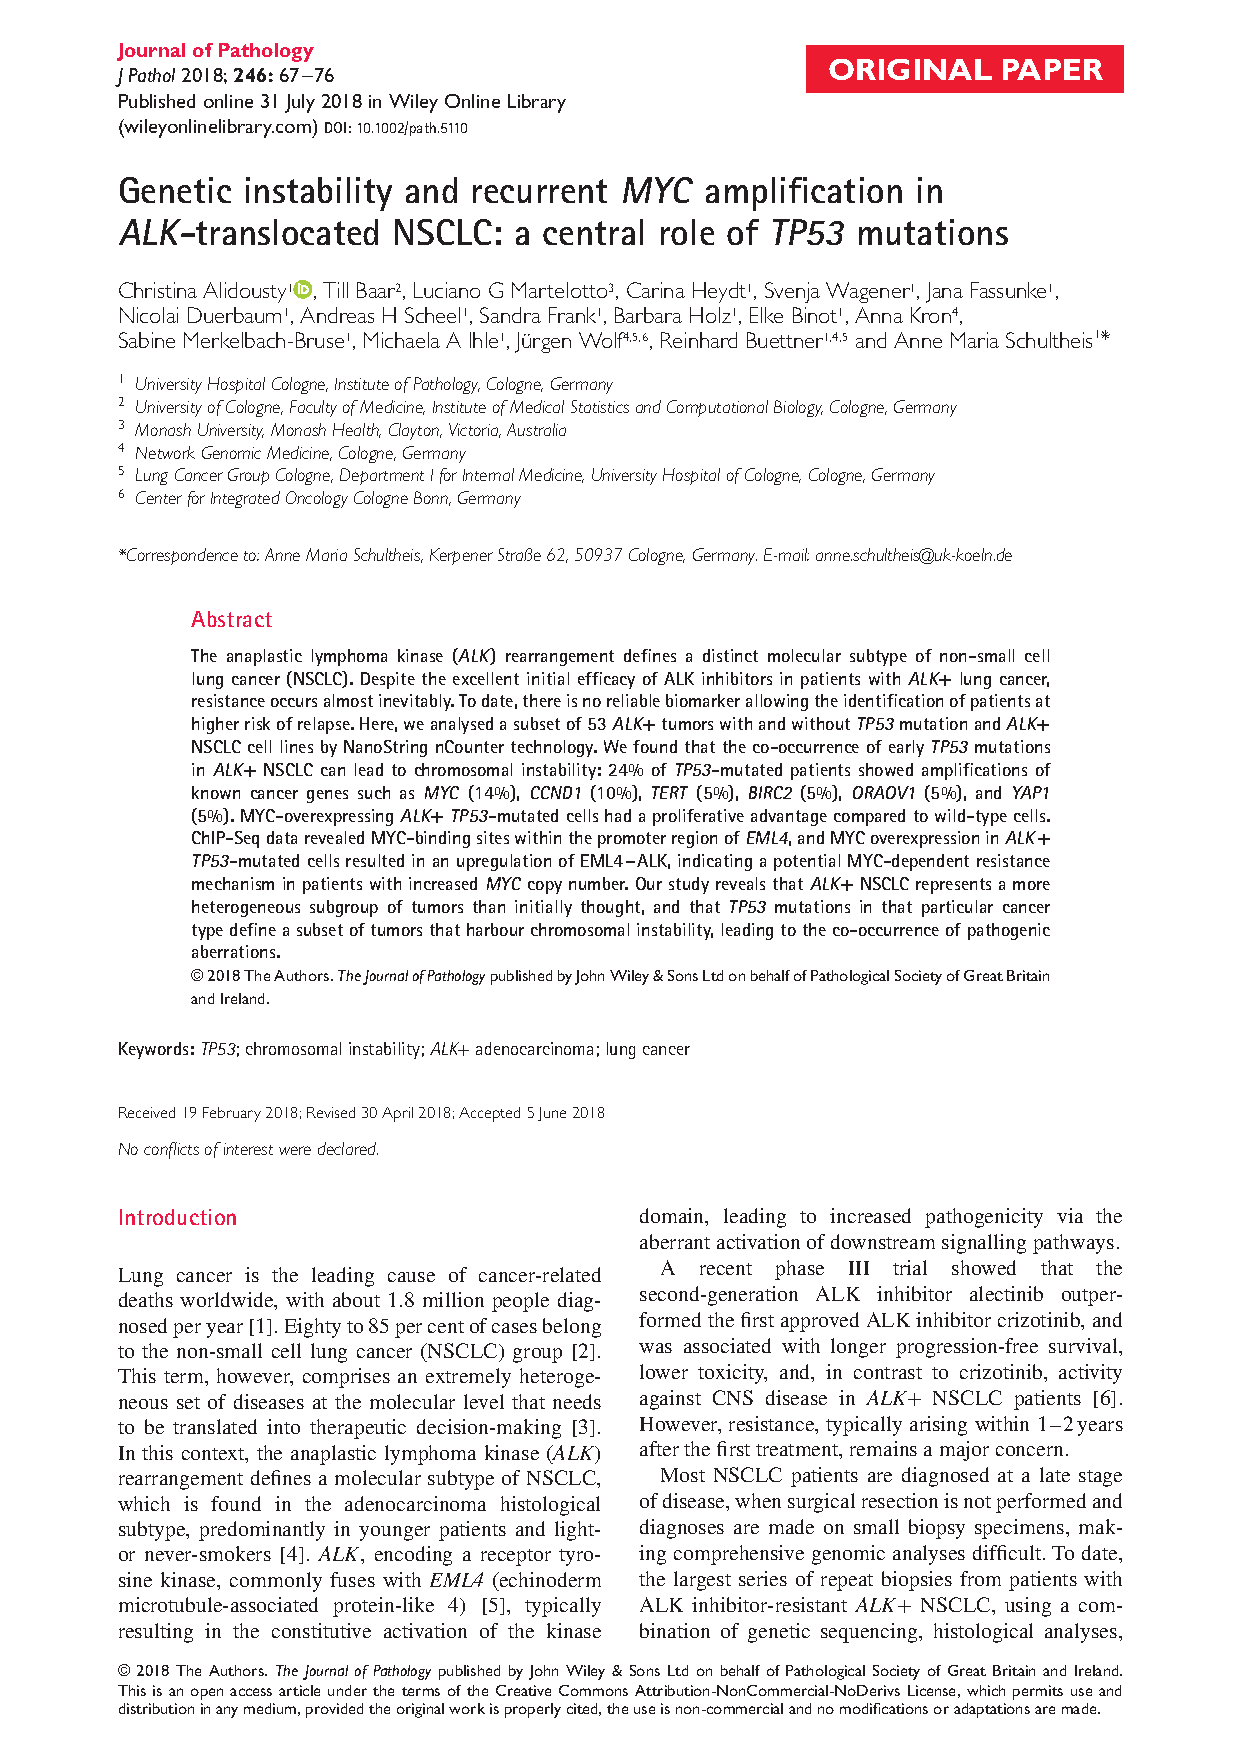
\includepdf[pages=-, addtotoc={1, section, 1,
  Genetic instability and recurrent MYC amplification in ALK-translocated
  NSCLC; a central role of TP53 mutations,
  Genetic instability and recurrent MYC amplification in ALK-translocated
  NSCLC; a central role of TP53 mutations}]
  {"99_Publications/Alidousty2018.pdf"}
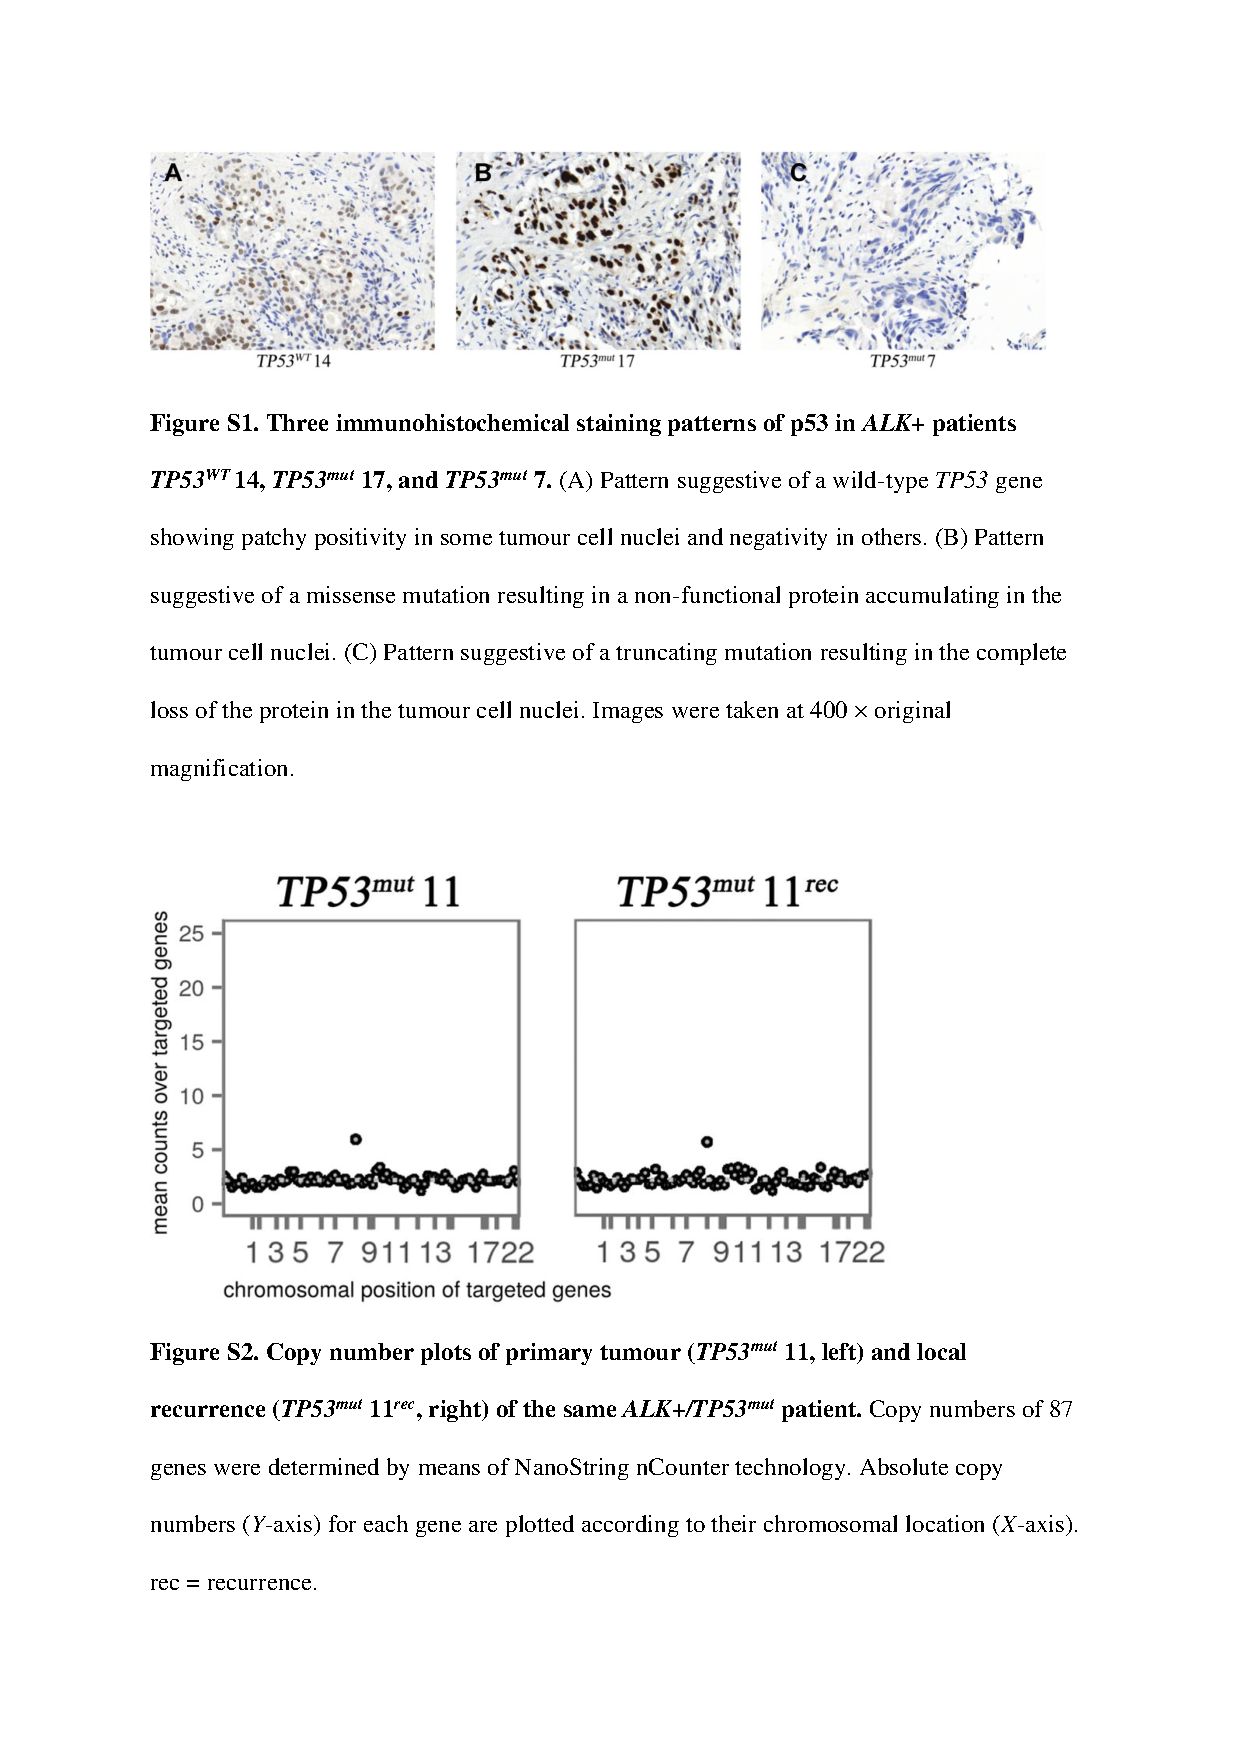
\includepdf[pages=-]{"99_Publications/Alidousty2018sup.pdf"}
% ┌────────────────────────────────────────────────────────────────────────────┐
% │ CONCLUSION                                                                 │
% └────────────────────────────────────────────────────────────────────────────┘

\chapter{Conclusion}

% ┌────────────────────────────────────────────────────────────────────────────┐
% │ END                                                                        │
% └────────────────────────────────────────────────────────────────────────────┘

% \chapter*{Introduction}
% An amalgamation of technological advancement and sophisticated magic offers many 
% amenities to the people of Ravnica (amenities that would be extraordinary to
% folk in more common fantasy settings). Almost all residential areas of the city
% enjoy central heating and plumbing, thanks to the work of the Izzet League, as
% well as elevators, and spacious apartments. There also exists an extensive
% public transport system, making every part of the city easily reachable.
% \begin{align*}
% t_{\nicefrac{1}{2}}=\frac{\ln\left(2\right)}{\delta}
% \end{align*}

% \section*{Section}
% Even poorer neighbourhoods boast clean and smooth roads and sturdy construction.
% No one needs to go hungry in Ravnica, because the Golgari Union provides a bare
% minimum of  sustenance to anyone who can't afford better food, though it is best
% not to think too much about where the thick gruel comes from. The citizens of
% Ravnica enjoy plenty of leisure time, as full-time employment in most cases
% means seven working hours per day, and the city offers an abundance of ways to
% fill it. Ravnica features restaurants with wide-ranging collections of fine
% wines, cafés serving coffee and tea, street vendors offering portable meals, and
% bakeries that sell a wide variety of breads and pastries \citep{Reich2013}.

% Travellers can stay in luxury hotels or simple hostels, or they can rely on
% their personal or guild-related contacts to find housing. \marginnote{This is a
% really long margin note that hopefully extends correctly over multiple lines.}
% Diversions and entertainments abound, including raucous street-side theatre,
% operas and symphonies, illegal fight clubs, sporting events held in vast
% arenas, throwaway popular novels, and great works of literature.

% \subsection*{Subsection}
% These things are shared by the city's diverse peoples, who enjoy a life adorned
% by a variety of  species, gender identities, and sexual orientations.
% Well-established systems undergird society, largely through the efforts of the
% guilds. The Azorius Senate crafts and codifies a comprehensive, though some
% would say oppressive, set of laws, enforced in turn by the Boros Corps. The Cult
% of Rakdos cares for the simple working class and criminal underworld, and the
% Golgari Union ensures that waste is disposed of and recycled. The Izzet League
% maintains the city's infrastructure, and the Orzhov Syndicate provides secure
% vaults and intricate financial arrangements, while their lawyers offer their
% services to anyone who can afford them. The Selesnya Conclave addresses issues
% of education and public health, as well as local public transport, while the
% Simic Combine sees to the biological maintenance and improvement of all
% citizens. \marginnote{This is a note}

% \subsubsection*{Subsubsection}
% Few parts of Ravnica could be considered wilderness. There exist abandoned sites
% where the infrastructure lies in ruins, partially reclaimed by natural forces.
% These are the only truly wild areas of the city, but even those do not last
% forever. It may take a hundred years or more, but sooner or later, these areas
% are reclaimed by civilization. In the meantime tough, they serve as safe havens
% for fugitives, malcontents, and failed, unlicensed experiments in
% thaumatological bioengineering that conveniently eloped from a Simic Combine
% research enclave.

% These things are shared by the city's diverse peoples, who enjoy a life adorned
% by a variety of  species, gender identities, and sexual orientations.
% Well-established systems undergird society, largely through the efforts of the
% guilds. The Azorius Senate crafts and codifies a comprehensive, though some
% would say oppressive, set of laws, enforced in turn by the Boros Corps. The Cult
% of Rakdos cares for the simple working class and criminal underworld, and the
% Golgari Union ensures that waste is disposed of and recycled. The Izzet League
% maintains the city's infrastructure, and the Orzhov Syndicate provides secure
% vaults and intricate financial arrangements, while their lawyers offer their
% services to anyone who can afford them. The Selesnya Conclave addresses issues
% of education and public health, as well as local public transport, while the
% Simic Combine sees to the biological maintenance and improvement of all
% citizens.

% These things are shared by the city's diverse peoples, who enjoy a life adorned
% by a variety of  species, gender identities, and sexual orientations.
% Well-established systems undergird society, largely through the efforts of the
% guilds. The Azorius Senate crafts and codifies a comprehensive, though some
% would say oppressive, set of laws, enforced in turn by the Boros Corps. The Cult
% of Rakdos cares for the simple working class and criminal underworld, and the
% Golgari Union ensures that waste is disposed of and recycled. The Izzet League
% maintains the city's infrastructure, and the Orzhov Syndicate provides secure
% vaults and intricate financial arrangements, while their lawyers offer their
% services to anyone who can afford them. The Selesnya Conclave addresses issues
% of education and public health, as well as local public transport, while the
% Simic Combine sees to the biological maintenance and improvement of all
% citizens.

% \chapter*{Methods}
% These things are shared by the city's diverse peoples, who enjoy a life adorned
% by a variety of  species, gender identities, and sexual orientations.
% Well-established systems undergird society, largely through the efforts of the
% guilds. The Azorius Senate crafts and codifies a comprehensive, though some
% would say oppressive, set of laws, enforced in turn by the Boros Corps. The Cult
% of Rakdos cares for the simple working class and criminal underworld, and the
% Golgari Union ensures that waste is disposed of and recycled. The Izzet League
% maintains the city's infrastructure, and the Orzhov Syndicate provides secure
% vaults and intricate financial arrangements, while their lawyers offer their
% services to anyone who can afford them. The Selesnya Conclave addresses issues
% of education and public health, as well as local public transport, while the
% Simic Combine sees to the biological maintenance and improvement of all
% citizens. \marginnote{text}

% These things are shared by the city's diverse peoples, who enjoy a life adorned
% by a variety of  species, gender identities, and sexual orientations.
% Well-established systems undergird society, largely through the efforts of the
% guilds. The Azorius Senate crafts and codifies a comprehensive, though some
% would say oppressive, set of laws, enforced in turn by the Boros Corps. The Cult
% of Rakdos cares for the simple working class and criminal underworld, and the
% Golgari Union ensures that waste is disposed of and recycled. The Izzet League
% maintains the city's infrastructure, and the Orzhov Syndicate provides secure
% vaults and intricate financial arrangements, while their lawyers offer their
% services to anyone who can afford them. The Selesnya Conclave addresses issues
% of education and public health, as well as local public transport, while the
% Simic Combine sees to the biological maintenance and improvement of all
% citizens.

% \begin{table}[t!]
% \caption[Currently available pathogen detection methods.]{This table lists six
% different currently available products to which the developed approach has been
% compared. Hybcell (Anagnostics) is a microarray-based diagnostic method which
% uses molecular markers to identify bacterial and fungal pathogens, and can also
% asses antibiotic resistance.}
% \begin{tabularx}{\textwidth}{llXcr}
%   Product   &             & Method     & Pathogens & Publication             \\
%   \midrule
%   Hybcell   & Anagnostics & microarray &           &                         \\
%   Prove-it  & Mobidiag    & microarray & 73        & \citealp{Aittakorpi2012}\\
%   SeptiFast & Roche       & PCR        & 25        & \citealp{Vince2008}     \\
%   SepsiTest & Molzym      & PCR        &           &                         \\
%   Unyvero   & Curetis     & microarray & 35        & \citealp{Jamal2014}     \\
%   VITEK     & bioMerieux  & culture    &           &                         \\
%   \bottomrule
% \end{tabularx}
% \label{tab:competitors}
% \end{table}

% These things are shared by the city's diverse peoples, who enjoy a life adorned
% by a variety of  species, gender identities, and sexual orientations.
% Well-established systems undergird society, largely through the efforts of the
% guilds. The Azorius Senate crafts and codifies a comprehensive, though some
% would say oppressive, set of laws, enforced in turn by the Boros Corps. The Cult
% of Rakdos cares for the simple working class and criminal underworld, and the
% Golgari Union ensures that waste is disposed of and recycled. The Izzet League
% maintains the city's infrastructure, and the Orzhov Syndicate provides secure
% vaults and intricate financial arrangements, while their lawyers offer their
% services to anyone who can afford them. The Selesnya Conclave addresses issues
% of education and public health, as well as local public transport, while the
% Simic Combine sees to the biological maintenance and improvement of all
% citizens.

% These things are shared by the city's diverse peoples, who enjoy a life adorned
% by a variety of  species, gender identities, and sexual orientations.
% Well-established systems undergird society, largely through the efforts of the
% guilds. The Azorius Senate crafts and codifies a comprehensive, though some
% would say oppressive, set of laws, enforced in turn by the Boros Corps. The Cult
% of Rakdos cares for the simple working class and criminal underworld, and the
% Golgari Union ensures that waste is disposed of and recycled. The Izzet League
% maintains the city's infrastructure, and the Orzhov Syndicate provides secure
% vaults and intricate financial arrangements, while their lawyers offer their
% services to anyone who can afford them. The Selesnya Conclave addresses issues
% of education and public health, as well as local public transport, while the
% Simic Combine sees to the biological maintenance and improvement of all
% citizens.

% These things are shared by the city's diverse peoples, who enjoy a life adorned
% by a variety of  species, gender identities, and sexual orientations
% \citep{Trapnell2010, Scholz2003, Schweitzer2011}. Well-established systems undergird society, largely
% through the efforts of the guilds. The Azorius Senate crafts and codifies a
% comprehensive, though some would say oppressive, set of laws, enforced in turn
% by the Boros Corps. The Cult of Rakdos cares for the simple working class and
% criminal underworld, and the Golgari Union ensures that waste is disposed of and
% recycled. The Izzet League maintains the city's infrastructure, and the Orzhov
% Syndicate provides secure vaults and intricate financial arrangements, while
% their lawyers offer their services to anyone who can afford them. The Selesnya
% Conclave addresses issues of education and public health, as well as local
% public transport, while the Simic Combine sees to the biological maintenance and
% improvement of all citizens.

% These things are shared by the city's diverse peoples, who enjoy a life adorned
% by a variety of  species, gender identities, and sexual orientations.
% Well-established systems undergird society, largely through the efforts of the
% guilds. The Azorius Senate crafts and codifies a comprehensive, though some
% would say oppressive, set of laws, enforced in turn by the Boros Corps. The Cult
% of Rakdos cares for the simple working class and criminal underworld, and the
% Golgari Union ensures that waste is disposed of and recycled. The Izzet League
% maintains the city's infrastructure, and the Orzhov Syndicate provides secure
% vaults and intricate financial arrangements, while their lawyers offer their
% services to anyone who can afford them. The Selesnya Conclave addresses issues
% of education and public health, as well as local public transport, while the
% Simic Combine sees to the biological maintenance and improvement of all
% citizens.

% \section*{Half-Life Estimation}

% Explanation of how we come to model the degradation rate
% $\delta$\marginnote{Usually, degradation rate is denoted by $\lambda$ not
% $\delta$, but the Poisson distribution's parameter is $\lambda$ already.} of Alu
% element transcripts. In our experiment, we measured Alu element expression using
% DTA (dynamic transcriptome analysis) with 4sU labelling. In this protocol, newly
% created transcripts are labelled, making them distinguishable from transcripts
% created before the labelling pulse. In the end, we want to obtain an estimate of
% the half-life $t_{\nicefrac{1}{2}}$ of each individual Alu element, which can be
% calculate from the degradation rate
% $\delta$ by
% \begin{equation*}
% t_{\nicefrac{1}{2}}=\frac{\ln\left(2\right)}{\delta}
% \end{equation*}

% \noindent The labelling pulse's duration $\Delta t$ is 5 min, meaning that 5 min
% passed after the labelling agent was added and before the amount of labelled
% transcripts within the cell was measured.

% With time, new transcripts are created and old transcript are degraded. This
% means that after the labelling pulse, the amount of unlabelled transcripts
% continually decreases, because all transcripts created after the labelling pulse
% are labelled, until only labelled transcripts remain. We assume that transcript
% degradation follows exponential decay, while the total amounts of transcripts
% in a cell remains constant, as transcription and transcript decay are in
% equilibrium. Therefore, the total amount of transcripts remains constant, but
% the ratio of labelled reads increases exponentially.

% \bigbreak
% \noindent\begin{minipage}{\textwidth}
% \centering
% % Created by tikzDevice version 0.12.3.1 on 2020-07-26 17:02:37
% !TEX encoding = UTF-8 Unicode
\begin{tikzpicture}[x=1pt,y=1pt]
\definecolor{fillColor}{RGB}{255,255,255}
\path[use as bounding box,fill=fillColor,fill opacity=0.00] (0,0) rectangle (180.67, 94.39);
\begin{scope}
\path[clip] ( 16.57,  0.00) rectangle (164.10, 94.39);
\definecolor{drawColor}{RGB}{255,255,255}
\definecolor{fillColor}{RGB}{255,255,255}

\path[draw=drawColor,line width= 0.5pt,line join=round,line cap=round,fill=fillColor] ( 16.57, -0.00) rectangle (164.10, 94.39);
\end{scope}
\begin{scope}
\path[clip] ( 41.40, 27.90) rectangle (159.10, 89.39);
\definecolor{fillColor}{RGB}{255,255,255}

\path[fill=fillColor] ( 41.40, 27.90) rectangle (159.10, 89.39);
\definecolor{drawColor}{RGB}{0,0,0}

\path[draw=drawColor,line width= 0.6pt,line join=round] ( 46.75, 30.69) --
	( 47.82, 33.44) --
	( 48.89, 36.05) --
	( 49.96, 38.53) --
	( 51.03, 40.89) --
	( 52.10, 43.14) --
	( 53.17, 45.28) --
	( 54.24, 47.31) --
	( 55.31, 49.25) --
	( 56.38, 51.09) --
	( 57.45, 52.84) --
	( 58.52, 54.50) --
	( 59.59, 56.08) --
	( 60.66, 57.59) --
	( 61.73, 59.02) --
	( 62.80, 60.39) --
	( 63.87, 61.68) --
	( 64.94, 62.92) --
	( 66.01, 64.09) --
	( 67.08, 65.20) --
	( 68.15, 66.27) --
	( 69.22, 67.28) --
	( 70.29, 68.24) --
	( 71.36, 69.15) --
	( 72.43, 70.02) --
	( 73.50, 70.85) --
	( 74.57, 71.63) --
	( 75.64, 72.38) --
	( 76.71, 73.09) --
	( 77.78, 73.77) --
	( 78.85, 74.41) --
	( 79.92, 75.03) --
	( 80.99, 75.61) --
	( 82.06, 76.16) --
	( 83.13, 76.69) --
	( 84.20, 77.19) --
	( 85.27, 77.67) --
	( 86.34, 78.12) --
	( 87.41, 78.55) --
	( 88.48, 78.96) --
	( 89.55, 79.35) --
	( 90.62, 79.73) --
	( 91.69, 80.08) --
	( 92.76, 80.41) --
	( 93.83, 80.73) --
	( 94.90, 81.04) --
	( 95.97, 81.33) --
	( 97.04, 81.60) --
	( 98.11, 81.86) --
	( 99.18, 82.11) --
	(100.25, 82.35) --
	(101.32, 82.58) --
	(102.39, 82.79) --
	(103.46, 82.99) --
	(104.53, 83.19) --
	(105.60, 83.37) --
	(106.67, 83.55) --
	(107.74, 83.71) --
	(108.81, 83.87) --
	(109.88, 84.02) --
	(110.95, 84.17) --
	(112.02, 84.30) --
	(113.09, 84.43) --
	(114.16, 84.56) --
	(115.23, 84.68) --
	(116.30, 84.79) --
	(117.37, 84.89) --
	(118.44, 85.00) --
	(119.51, 85.09) --
	(120.58, 85.18) --
	(121.65, 85.27) --
	(122.72, 85.35) --
	(123.79, 85.43) --
	(124.86, 85.51) --
	(125.93, 85.58) --
	(127.00, 85.65) --
	(128.07, 85.71) --
	(129.14, 85.77) --
	(130.21, 85.83) --
	(131.28, 85.89) --
	(132.35, 85.94) --
	(133.42, 85.99) --
	(134.49, 86.04) --
	(135.56, 86.08) --
	(136.63, 86.13) --
	(137.70, 86.17) --
	(138.77, 86.21) --
	(139.84, 86.24) --
	(140.91, 86.28) --
	(141.98, 86.31) --
	(143.05, 86.35) --
	(144.12, 86.38) --
	(145.19, 86.40) --
	(146.26, 86.43) --
	(147.33, 86.46) --
	(148.40, 86.48) --
	(149.47, 86.51) --
	(150.54, 86.53) --
	(151.61, 86.55) --
	(152.68, 86.57) --
	(153.75, 86.59);

\path[draw=drawColor,line width= 0.5pt,line join=round,line cap=round] ( 41.40, 27.90) rectangle (159.10, 89.39);
\end{scope}
\begin{scope}
\path[clip] (  0.00,  0.00) rectangle (180.67, 94.39);
\definecolor{drawColor}{RGB}{0,0,0}

\node[text=drawColor,anchor=base east,inner sep=0pt, outer sep=0pt, scale=  0.80] at ( 36.90, 27.94) {0};

\node[text=drawColor,anchor=base east,inner sep=0pt, outer sep=0pt, scale=  0.80] at ( 36.90, 84.22) {1};
\end{scope}
\begin{scope}
\path[clip] (  0.00,  0.00) rectangle (180.67, 94.39);
\definecolor{drawColor}{RGB}{0,0,0}

\path[draw=drawColor,line width= 0.3pt,line join=round] ( 38.90, 30.69) --
	( 41.40, 30.69);

\path[draw=drawColor,line width= 0.3pt,line join=round] ( 38.90, 86.97) --
	( 41.40, 86.97);
\end{scope}
\begin{scope}
\path[clip] (  0.00,  0.00) rectangle (180.67, 94.39);
\definecolor{drawColor}{RGB}{0,0,0}

\path[draw=drawColor,line width= 0.3pt,line join=round] ( 46.75, 25.40) --
	( 46.75, 27.90);

\path[draw=drawColor,line width= 0.3pt,line join=round] (153.75, 25.40) --
	(153.75, 27.90);
\end{scope}
\begin{scope}
\path[clip] (  0.00,  0.00) rectangle (180.67, 94.39);
\definecolor{drawColor}{RGB}{0,0,0}

\node[text=drawColor,anchor=base,inner sep=0pt, outer sep=0pt, scale=  0.80] at ( 46.75, 17.89) {0};

\node[text=drawColor,anchor=base,inner sep=0pt, outer sep=0pt, scale=  0.80] at (153.75, 17.89) {t};
\end{scope}
\begin{scope}
\path[clip] (  0.00,  0.00) rectangle (180.67, 94.39);
\definecolor{drawColor}{RGB}{0,0,0}

\node[text=drawColor,anchor=base,inner sep=0pt, outer sep=0pt, scale=  1.00] at (100.25,  6.94) {Time};
\end{scope}
\begin{scope}
\path[clip] (  0.00,  0.00) rectangle (180.67, 94.39);
\definecolor{drawColor}{RGB}{0,0,0}

\node[text=drawColor,rotate= 90.00,anchor=base,inner sep=0pt, outer sep=0pt, scale=  1.00] at ( 28.46, 58.64) {L / T};
\end{scope}
\end{tikzpicture}

% \vspace{-\ht\strutbox}
% \captionof{figure}[Exponential RNA degradation]{Model illustration of the
% exponential RNA degradation and the resulting $L/T$ ratio over time.}
% \label{fig:expdecay}
% \end{minipage}
% \bigbreak

% \noindent Let $t_{a}$ be the total number of molecules of any Alu element $a$ in
% solution. Among those $t_{a}$ molecules, let $l_{a}$ denote the number of newly
% synthesized (and therefore labelled) molecules. By assumption of steady state
% conditions and an exponential decay, the ratio between labelled and total
% molecules $r_{a}$ for any Alu element $a$ is given by
% \begin{align*}
%   r_{a}     &= \nicefrac{l_{a}}{t_{a}}=1-\exp(-\delta_{g}\Delta t)
% \\ \ln r_{a} &= \ln\left(1-\exp(-\delta_{g}\Delta t)\right)
% \end{align*}

% \noindent where $\delta_{a}$ is the degradation rate of any Alu element $a$. The
% total amount of molecules $t_{a}$ of any Alu element $a$ is also given as:
% \begin{equation*}
% t_{a}=\nicefrac{\mu_{a}}{\delta_{a}}
% \end{equation*}

% \noindent where $\mu_{a}$ is the synthesis rate of any Alu element $a$.

% \noindent\marginnote{This approximation could be replaced by the solution of the
% standard ODE for RNA metabolism, or by a term that takes into account the
% non-constant labelling efficiency for short labelling periods.}Neglecting the
% decay of newly synthesized transcripts, we likewise obtain
% \begin{equation*}
% l_{a}=\mu_{a}\Delta t
% \end{equation*}

% \noindent We further assume that
% \begin{equation*}
% l_{all}=\sum_{a}l_{a}\quad\text{and}\quad t_{all}=\sum_{a}t_{a}
% \end{equation*}

% \noindent We now shift our view from the molecules in solution to read counts
% obtained through sequencing. We prepare a sequencing library with $N_{tot}$
% reads. After 4sU pull-down, we prepare a sequencing library of size $N_{lab}$
% reads. The distribution of total counts $T_{a}$ and labelled counts $L_{a}$
% respectively for any Alu element $a$ is then\marginnote{There is also the
% possibility to choose a (zero-inflated) negative binomial distribution instead.}
% \begin{align*}
%   T_{a} &\sim \operatorname{Pois}
%   (\lambda_{tot}=\frac{t_{a}}{t_{all}}\cdot N_{tot})
% \\ L_{a} &\sim \operatorname{Pois}
%   (\lambda_{lab}=\frac{l_{a}}{l_{all}}\cdot N_{lab})
% \end{align*}

% \noindent We thus assume that the estimated ratio between labelled and total
% molecules $\hat{r}_{a}$ for any Alu element $a$ is given by
% \begin{equation*}
% \hat{r}_{a}=\frac{L_{a}}{T_{a}}\cdot\frac{N_{tot}}{N_{lab}}
% \end{equation*}

% \noindent We still need to estimate $\nicefrac{l_{all}}{t_{all}}$ i.e., the
% fraction of (all) labelled molecules among all molecules in solution. We use
% spike-ins to do so. Let $l_{\text{spk}}$ be the number of labelled spike-in
% molecules, and $t_{\text{spk}}$ the number of total spike-in molecules that were
% added to the solution. We know that
% \begin{equation}
% \frac{l_{spk}}{l_{all}}\approx\frac{L_{spk}}{L_{all}}=\frac{L_{spk}}{N_{lab}}
% \quad\text{and}\quad
% \frac{t_{spk}}{t_{all}}\approx\frac{T_{spk}}{T_{all}}=\frac{T_{spk}}{N_{tot}}
% \label{spk}
% \end{equation}

% \noindent The term $q=\nicefrac{l_{spk}}{t_{spk}}$ is thus known by composition
% of the spike-in reagents.

% \listoffigures

% \listoftables

\bibliographystyle{07_Bibliography/urlapa}        % defines bibliography style
\bibliography{07_Bibliography/library}            % bibtex file location

\cleardoublepage

\begin{otherlanguage}{german}

\chapter*{Erkl\"arung zur Dissertation}
\addcontentsline{toc}{subsection}{Erkl\"arung (Statement)}

Hiermit versichere ich an Eides statt, dass ich die vorliegende Dissertation
selbstständig und ohne die Benutzung anderer als der angegebenen Hilfsmittel
und Literatur angefertigt habe. Alle Stellen, die wörtlich oder sinngemäß aus
veröffentlichten und nicht veröffentlichten Werken dem Wortlaut oder dem Sinn
nach entnommen wurden, sind als solche kenntlich gemacht. Ich versichere an
Eides statt, dass diese Dissertation noch keiner anderen Fakultät oder
Universität zur Prüfung vorgelegen hat; dass sie -- abgesehen von unten
angegebenen Teilpublikationen und eingebundenen Artikeln und Manuskripten --
noch nicht veröffentlicht worden ist sowie, dass ich eine Veröffentlichung der
Dissertation vor Abschluss der Promotion nicht ohne Genehmigung des
Promotionsausschusses vornehmen werde. Die Bestimmungen dieser Ordnung sind mir
bekannt. Darüber hinaus erkläre ich hiermit, dass ich die Ordnung zur
Sicherung guter wissenschaftlicher Praxis und zum Umgang mit wissenschaftlichem
Fehlverhalten der Universität zu Köln gelesen und sie bei der Durchführung der
Dissertation zugrundeliegenden Arbeiten und der schriftlich verfassten
Dissertation beachtet habe und verpflichte mich hiermit, die dort genannten
Vorgaben bei allen wissenschaftlichen Tätigkeiten zu beachten und umzusetzen.
Ich versichere, dass die eingereichte elektronische Fassung der eingereichten
Druckfassung vollständig entspricht.

\vspace{5\baselineskip}
\hrule
\vspace{\dp\strutbox}

Till Baar

\end{otherlanguage}

\cleardoublepage

\cleardoublepage

\begin{otherlanguage}{german}

\chapter*{Lebenslauf}
\addcontentsline{toc}{subsection}{Lebenslauf (Curriculum Vitae)}

{\LARGE Till Baar}

\vspace{\baselineskip}

\noindent 28.12.1987, Hamburg \hfill (Deutsche Staatsangehörigkeit)

\vspace{0.5\baselineskip}

\noindent Steinstraße 32, 52372 Kreuzau

\vspace{0.5\baselineskip}

\noindent\textbf{Schulische Ausbildung}\dotfill

\vspace{0.5\baselineskip}

\renewcommand{\arraystretch}{1.25}
\noindent\begin{tabularx}{\textwidth}{rcX}
1994 -- 1998 & & Grundschule Schortens \\
1998 -- 2000 & & Franziskusschule Wilhelmshaven (OS) \\
2000 -- 2007 & & Cäcilienschule Wilhelmshaven \newline freies Gymnasium in
                 kirchl. Trägerschaft \newline
                 \hspace*{\fill} (Abschluss:~Abitur) \\
\end{tabularx}

\vspace{\dp\strutbox}
\noindent\dotfill
\vspace{\dp\strutbox}

\noindent\begin{tabularx}{\textwidth}{rcX}
2007 -- 2008 & & Zivildienst, FöJ Tierpark Bochum \\
\end{tabularx}

\vspace{\dp\strutbox}
\noindent\textbf{Universitäre Ausbildung}\dotfill
\vspace{\dp\strutbox}

\noindent\begin{tabularx}{\textwidth}{rcX}
2008 -- 2009 & & Bachelor Studiengang Geophysik / Meteorologie, Universität zu
                 Köln \\
2009 -- 2012 & & Bachelor Studiengang Biologie, Universität zu Köln
                 \hfill (Abschluss:~B.Sc.) \\
2013 -- 2015 & & Master Studiengang Biological Sciences, Universität zu Köln
                 \hfill (Abschluss:~M.Sc.) \\
2015 -- 2017 & & Wiss. Mitarbeiter Molekularpathologie, Institut für
                 Pathologie, Universitätsklinikum Köln \\
2017 -- 2022 & & Wiss. Mitarbeiter AG Computational Biology, IMSB, Fakulät für
                 Medizin, Universität zu Köln \hfill (Promotion) \\
\end{tabularx}


\vfill
\hrule
\vspace{\dp\strutbox}

Till Baar

\end{otherlanguage}

\chapter*{Acknowledgements}
\addcontentsline{toc}{chapter}{Acknowledgements}

Throughout my doctoral studies, I have received a great deal of support and
assistance.

\bigbreak
\noindent I would first and foremost like to thank my supervisor, Prof. Dr.
Achim Tresch, whose expertise was invaluable in formulating my research
questions and methodology. His insightful feedback pushed me to sharpen my
thinking and brought my work to a higher level. He was instrumental in
defining the path of my research, and for his guidance through each stage of
my doctoral studies, I am immensely grateful.

\bigbreak
\noindent My heartfelt thanks also go out to the many excellent scientists
that collaborated with me on the publications included in my dissertation.

\bigbreak
\noindent I would also like to thank my colleagues at the Institute of Medical
Statistics and Computational Biology, and the Computational Biology workgroup
in particular, for their wonderful fellowship. The companionable atmosphere in
our office makes every day I spend with them a pleasure.

\bigbreak
\noindent Furthermore, without the support of Prof. Dr. Michael Melkonian,
Prof. Dr. Günter Plickert, and Dr. Lisa Stephan in my early course of
studies, I would not have made it this far.

\bigbreak
\noindent Moreover, I would like to thank my parents, who always believed in
my ability to be successful in academia. None of this would have been possible
without them and their unending encouragement, for which I am grateful beyond
words. I know that they could hardly be any prouder of me, but I hope they
take delight in knowing that my small contributions to the sum total of human
knowledge bear their subtle brushstrokes, too.

\bigbreak
\noindent Finally, I could not have completed my dissertation without the
support of all of my friends, especially Peter and Dave, who provided
invaluable support, stimulating discussions, as well as the essential
distraction to rest my mind outside of research.

% ┌────────────────────────────────────────────────────────────────────────────┐
% │ RRZK                                                                       │
% └────────────────────────────────────────────────────────────────────────────┘

\newpage\null\vfill
\sectionmark{Acknowledgements}
\noindent I thank the Regional Computing Center of the University of Cologne
(RRZK) for providing computing time on the DFG-funded (Funding number: INST
216\thinspace{}/\thinspace{}512\thinspace{}/\thinspace{}1FUGG) High
Performance Computing (HPC) system CHEOPS as well as support.
\vfill 

\end{document}